\documentclass[class=article , crop=false, titlepage, twoside, multi={itemize, figure, verbatim}, float=false]{standalone}

\usepackage{import} % Required for importing other .tex docs.  (import uses everything bw Begin and End Doc)
\usepackage{float} % Required for specifying the exact location of a figure or table
\usepackage{graphicx} % Required for including images
\usepackage{wrapfig}
\usepackage[pdftex,breaklinks,colorlinks=true,linkcolor=black,citecolor=blue,urlcolor=red,linktocpage=false,pagebackref=true,filecolor=magenta]{hyperref}%http://www.tug.org/applications/hyperref/manual.html#x1-100003.6
\usepackage{cite}
\usepackage[toc,title,page]{appendix}
\usepackage{pdfpages} % enables loading a pdf into the doc
\usepackage{makeidx}
\usepackage{glossaries} % must be after hyperref
\usepackage{blindtext}
\usepackage{enumitem}
%\usepackage{caption}

%\setlist[description]{leftmargin=\parindent,labelindent=\parindent}

%\renewcommand*{\bibname}{References} % renames the bibliography

\newcommand{\HRule}{\rule{\linewidth}{0.5mm}} % Command to make the lines in the title page

\graphicspath{{img/}{GIS_ChampionSection/img/}{awardsChapter/GIS_ChampionSection/img/}{brandPart/awardsChapter/GIS_ChampionSection/img/}{img/}{pairedProgSection/img/}{methodChapter/pairedProgSection/img/}{methodPart/methodChapter/pairedProgSection/img/}{documentationSection/img/}{methodChapter/documentationSection/img/}{methodPart/methodChapter/documentationSection/img/}{docStorageOrgSection/img/}{methodChapter/docStorageOrgSection/img/}{methodPart/methodChapter/docStorageOrgSection/img/}{QGisSection/img/}{toolsChapter/QGisSection/img/}{servicePart/toolsChapter/QGisSection/img/}{ESRISection/img/}{toolChapter/ESRISection/img/}{servicePart/toolChapter/ESRISection/img/}{../../../../source/}{../../source/}{servicePart/applicationsChapter/treasurerSection/img/}}

%\setlength\parindent{0pt} % eliminates indents


\def\titlename{Forfeiture Data Collection\\ \medskip\large Mobile App with Collector for ArcGIS}

\title{\HRule % Horizontal Line added
\\[.4cm] % space
\begin{figure}[H] % included image
\begin{center}	% centered horizontally
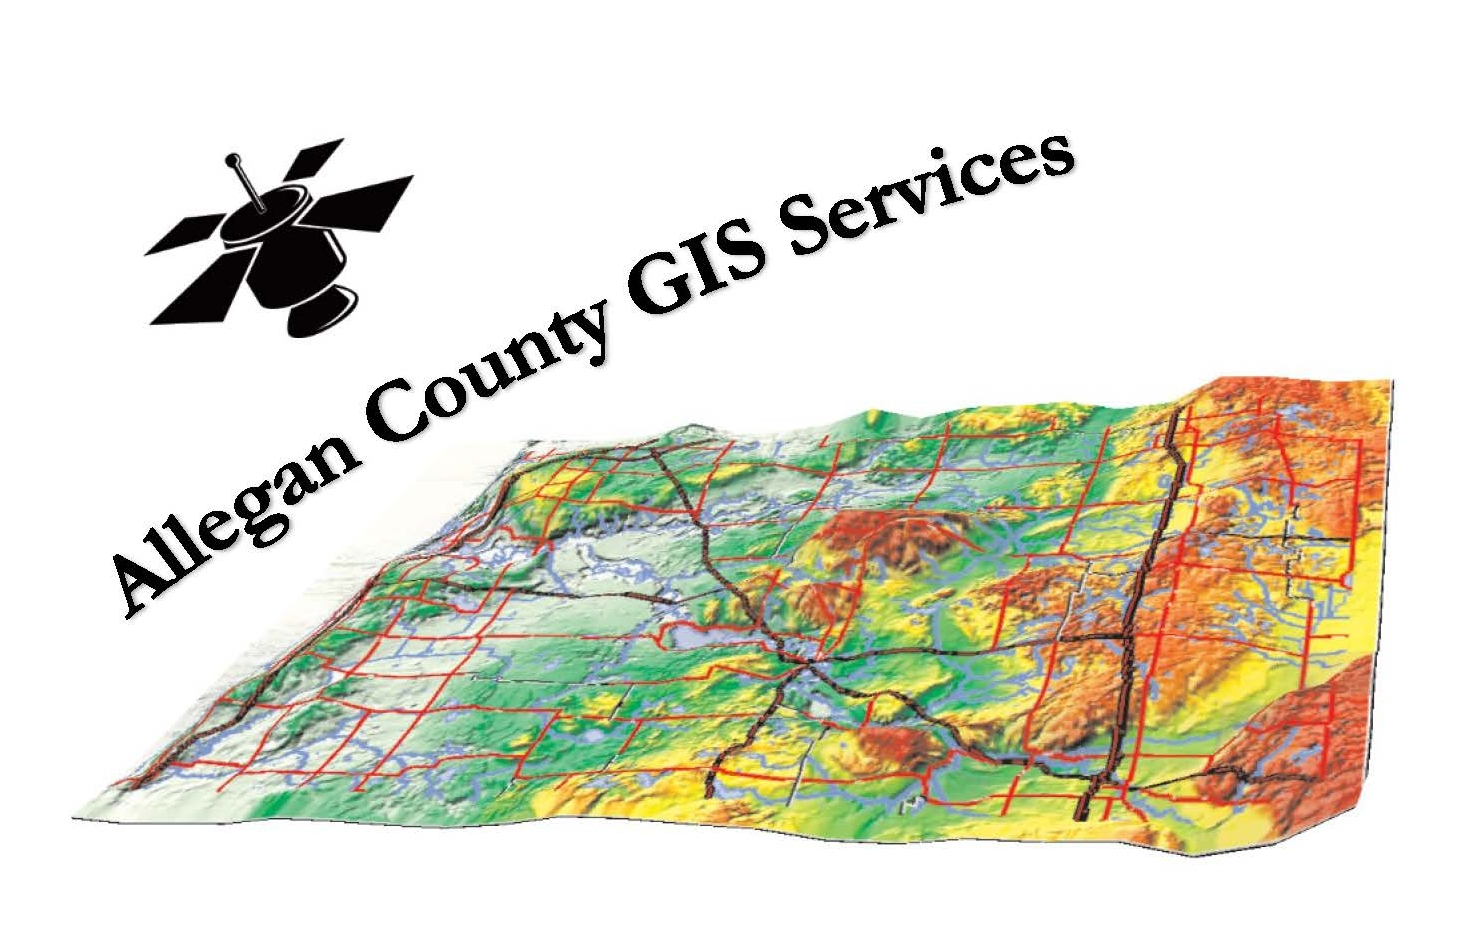
\includegraphics[scale=.45]{GIS_Logo_better.jpg}
\end{center}
\end{figure}
\Huge \bfseries \titlename \\ % Title text
\HRule \\[.4cm] % Horizontal Line added
\author{\Large Allegan County GIS \\\Large www.allegancounty.org/gis} % defines author
}  % inputs common title
\setcounter{tocdepth}{5}  % subparagraph and down
\begin{document}% document begins

\ifstandalone
\maketitle % creates title page
\clearpage
\tableofcontents % creates TOC
\clearpage
\fi

\subsection{Forfeiture Data Collection}

\subsubsection{Problem and Analysis}

\paragraph{Background}
Treasurer department has an annual responsibility to properly document the tax forfeiture process.  The LIS Department built an application in MS Access and MapInfo that consumed a daily export from BSA and was deployed to the field on a laptop.  A digital camera was used for site photos and later imported into the laptop.

\paragraph{Statement of Problem}
Current Tax Forfeiture workflow is built on MapInfo software which has been replaced by ESRI software.  The Forfeiture data collection application must be recreated in the ESRI framework.

\paragraph{Analysis}
Tax Forfeiture Application will facilitate:

\begin{itemize} %1

\item Mobile data collection on handheld device via Collector for ArcGIS configured with Allegan County GIS Portal  (\textbf{device app})

\begin{itemize} %2

\item Device app will:

\begin{itemize} %3

\item Synchronize with data in the office (online)
\item Navigate to forfeiture sites (offline)
\item Collect data and photos of forfeiture sites (offline)
\item Synchronize the collected data with data in the office (online)
\end{itemize} %3

\end{itemize} %2

\item Daily form production and printing for each site visited with required data and images.

\end{itemize} %1

\clearpage
\subsubsection{Design}
\paragraph{Overview}This Application utilizes Treasurer Department data to document the forfeiture process.  An enterprise GIS deployment enables offline data collection by up to two users.
\begin{figure}[h!]
\centering
    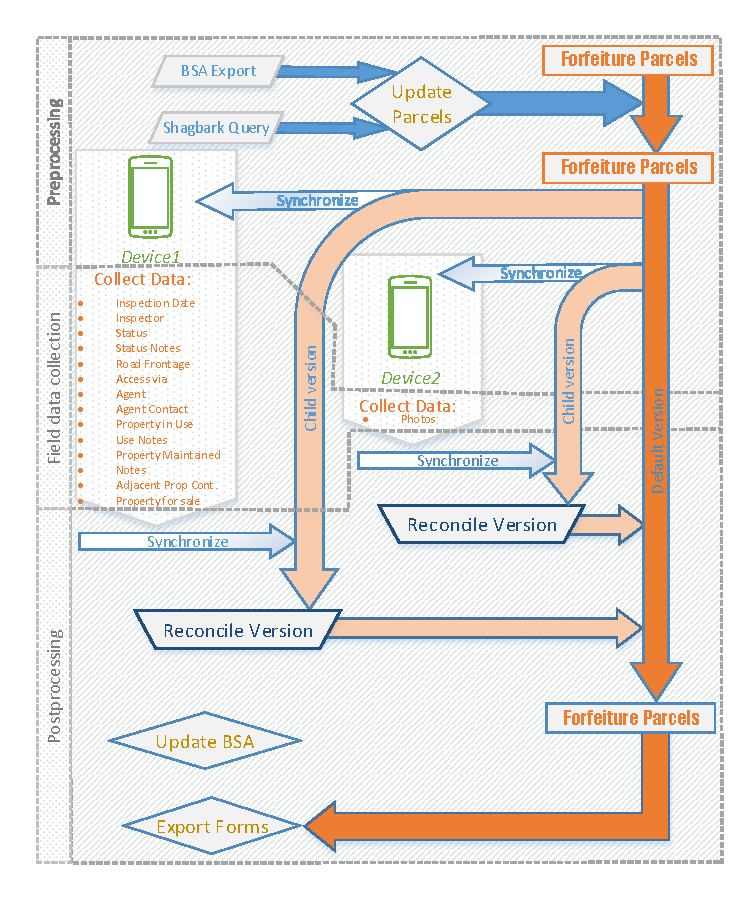
\includegraphics[width=.95\textwidth]{ProjectDesign}
    %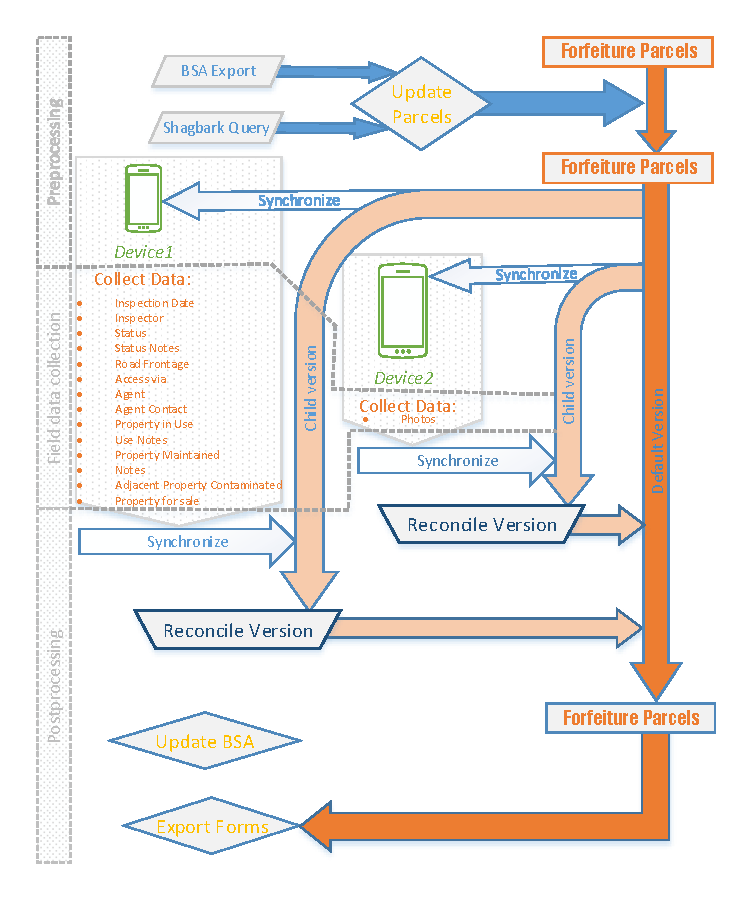
\includegraphics{DesignFlowChart}
\caption{Project Design}
\end{figure}
\subparagraph*{}There are three stages to daily workflow: Preprocessing, Field Collection, and Postprocessing.  Forfeiture Parcels, is a map feature class that is processed in the office via the network and remotely via the internet.
\clearpage
\subparagraph{Workflow Summary}
\begin{description}
\item [Preprocessing] The data is updated to match the Treasures data in BSAforfeiture.net and synchronized to two android mobile devices.
\item [Field data collection] The two mobile devices are used to collect info required, one for all the attributes, the other for photos.
\item[Postprocessing] The mobile devices are syncronized back to the network data and a form is exported for each site visited that day.
\end{description}


\paragraph{Technologies Used}
\subparagraph{BSA Data}Details of parcels in the forfeiture process are managed in BSA Delinquent Tax.net.  The Treasurer office does a BSA export of the parcels in need of a site visit in the preprocessing.

\subparagraph{ArcGIS Desktop}Tools are designed to preprocess and postprocess forfeiture parcel data for fieldwork.  The user will execute a preprocess script tool that prepares the data for field deployment.  After fieldwork, a post process script tool syncronizes data from the fieldwork with the live data on the Allegan County network. 

\subparagraph{ArcGIS Collector}A free mobile application developed and tested on Android is deployed to the field for data collection.  The application is configured to work offline(without an internet or cellular connection) by syncronizing before and after fieldwork.

\subparagraph{ArcGIS Portal Webmaps and Apps}Live data from a publishing enterprise geodatabase(ACPub), running on SQL Server database server (acintsql01) is provided through a feature service (REST service)  named TaxReversionParcels.  A webmap called the Forfeiture Field Map consumes the TaxReversionParcels feature service, exposing the data to editing.  The Forfeiture Field Map is configured to work in the ArcGIS Collector App.  The app downloads the webmap, allowing the user to collect the necessary information on each forfeiture parcel in the field disconnected and uploads the changes when reconnected. 

\paragraph{Field Data Collection}

Three parts of the daily routine:
\begin{enumerate}
\item Pre-processing (in the office):

\begin{itemize}
\item Export current forfeiture list from BSA
\item Update webmap layers with results from BSA export
\item Synchronize from webmap layers to field collection devices \textbf{(device app)}
\end{itemize}

\item Field data collection with device app:

\begin{itemize}
\item Navigation to forfeiture sites is aided by users location shown in map
\item A Checklist of data points about the site
\item Attach photos to the site
\item Save results for synchronization in post-processing
\end{itemize}

\item Post-processing (in the office)

\begin{itemize}
\item Synchronize data and images collected in device app to webmap layers

\end{itemize}
\end{enumerate}

\paragraph{Data Details}
\subparagraph{Location of Production Data}
\begin{wrapfigure}{r}{0.5\textwidth}
\centering
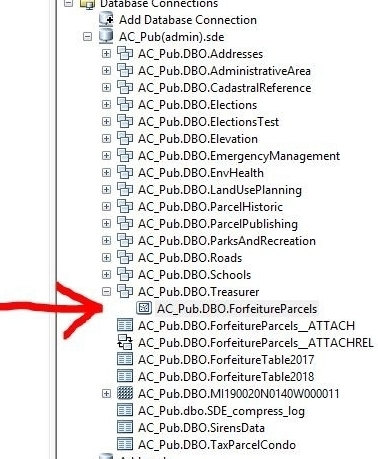
\includegraphics[width=.45\textwidth]{LiveDataLocationScreenshot}
\caption{Live Data Location Screenshot}
\end{wrapfigure}
The data is located in ACPUB.
\clearpage

\subparagraph{ForfeitureParcels Feature Class}

\paragraph{Collector for ArcGIS}

\clearpage
\paragraph{Webmap Details}

\clearpage
\subsubsection{Hard Copy Record}


\clearpage
\subsubsection{User Manual}

\paragraph{Admin Tasks}

\subparagraph{Setup Users in ArcGIS}Users that will run Pre and Post processing scripts must be created and given priviliges on ACPub Treasurer Feature Data Set.

\subparagraph{Setup Users in Portal for ArcGIS}Users that will use the Collector for ArcGIS must have profiles added to and managed in the Allegan County GIS Portal site.

\subparagraph{Schema Change Procedure}

\subparagraph{Form Edits Procedure}

\paragraph{Collection Device Setup}

\subparagraph{Camera Settings}

\subparagraph{Internet Settings}

\clearpage
\paragraph{Collector Setup Details}

\subparagraph{Install Collector for ArcGIS}
\begin{itemize}
\item Available from the Google Play Store
\end{itemize}
\begin{figure}[h!]
\centering
    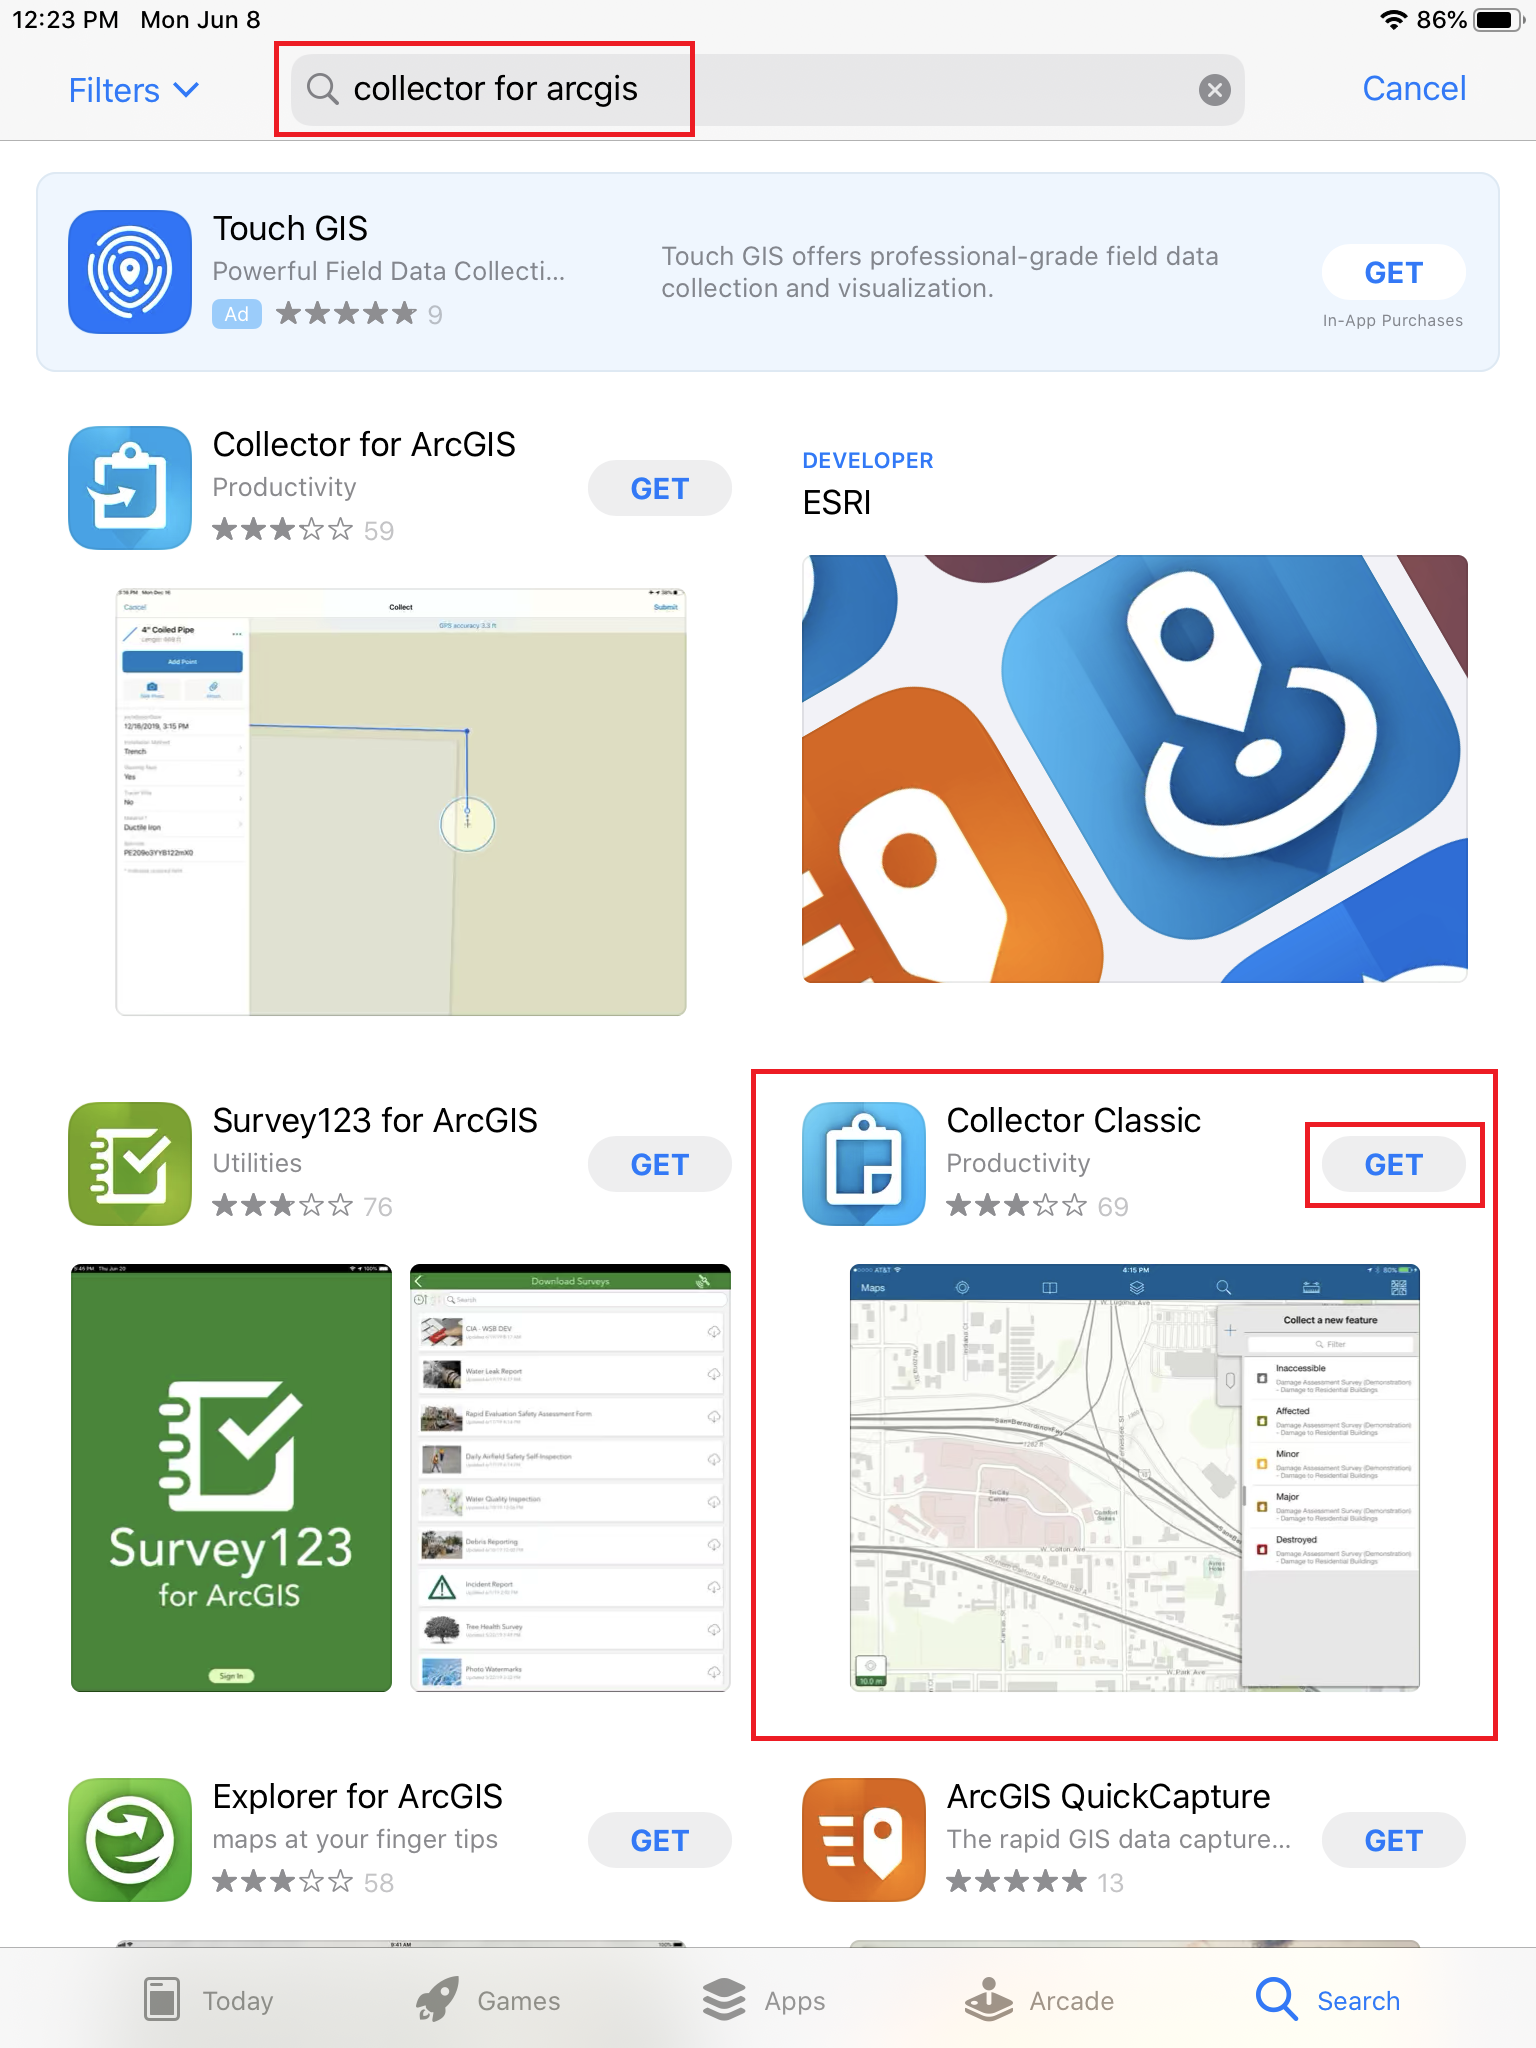
\includegraphics[width=.5\textwidth]{DownloadtheApp.png}
\caption{Download the App}
\end{figure}

\clearpage
\subparagraph{Configure Collector}

\subparagraph*{\\}
\begin{wrapfigure}{r}{0.5\textwidth}
\centering
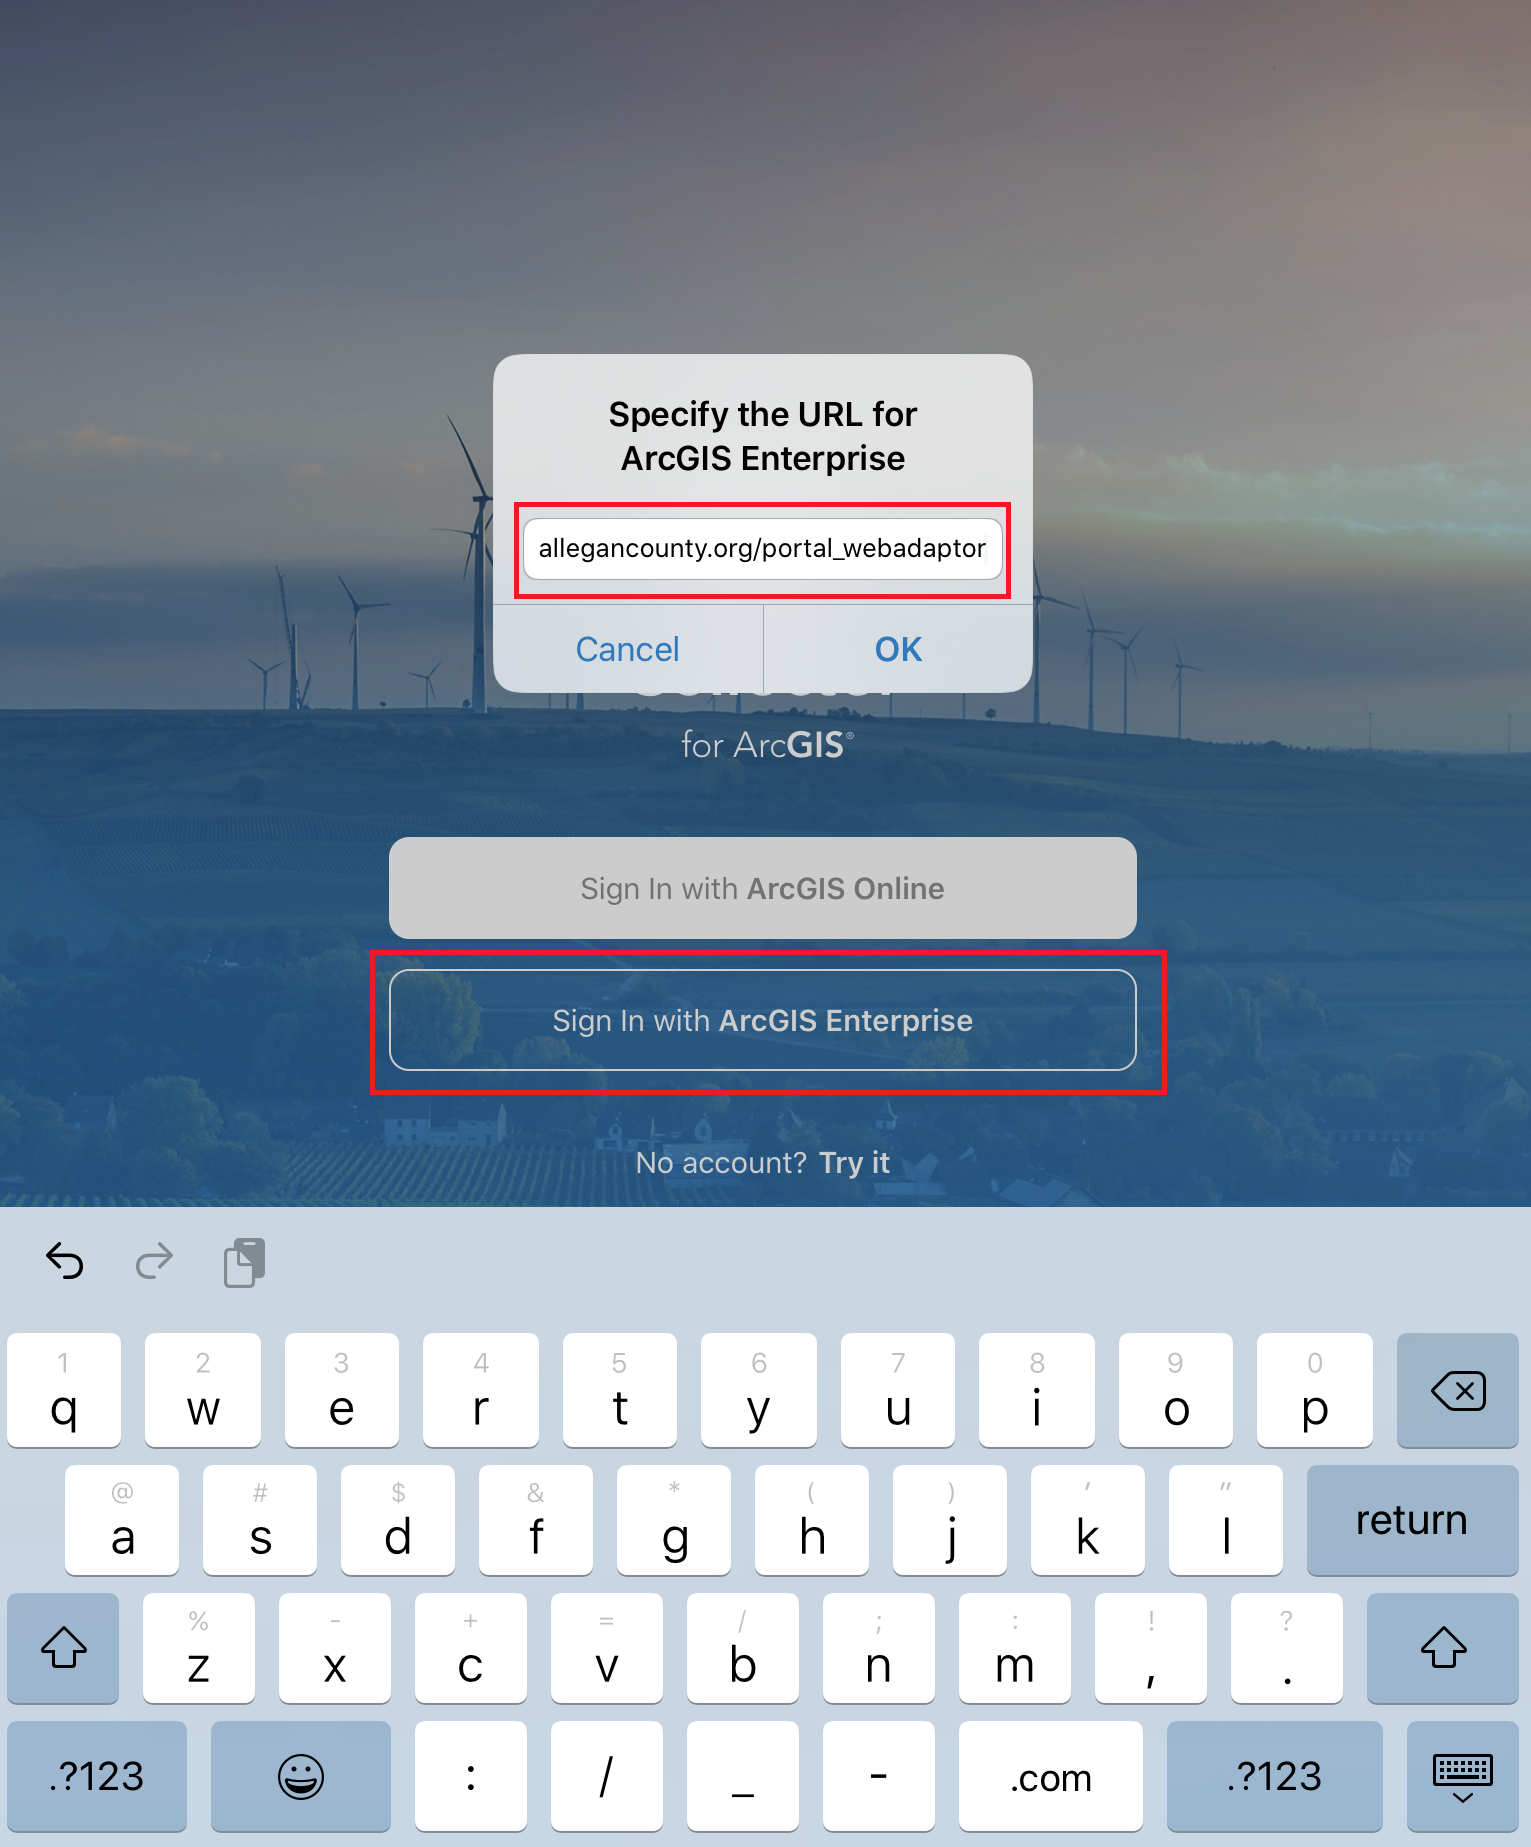
\includegraphics[width=.3\textwidth]{CollectorConnection}
\caption{Collector Connection}
\vspace{.25in}
\HRule \\[.4cm] % Horizontal Line added
\vspace{.25in}
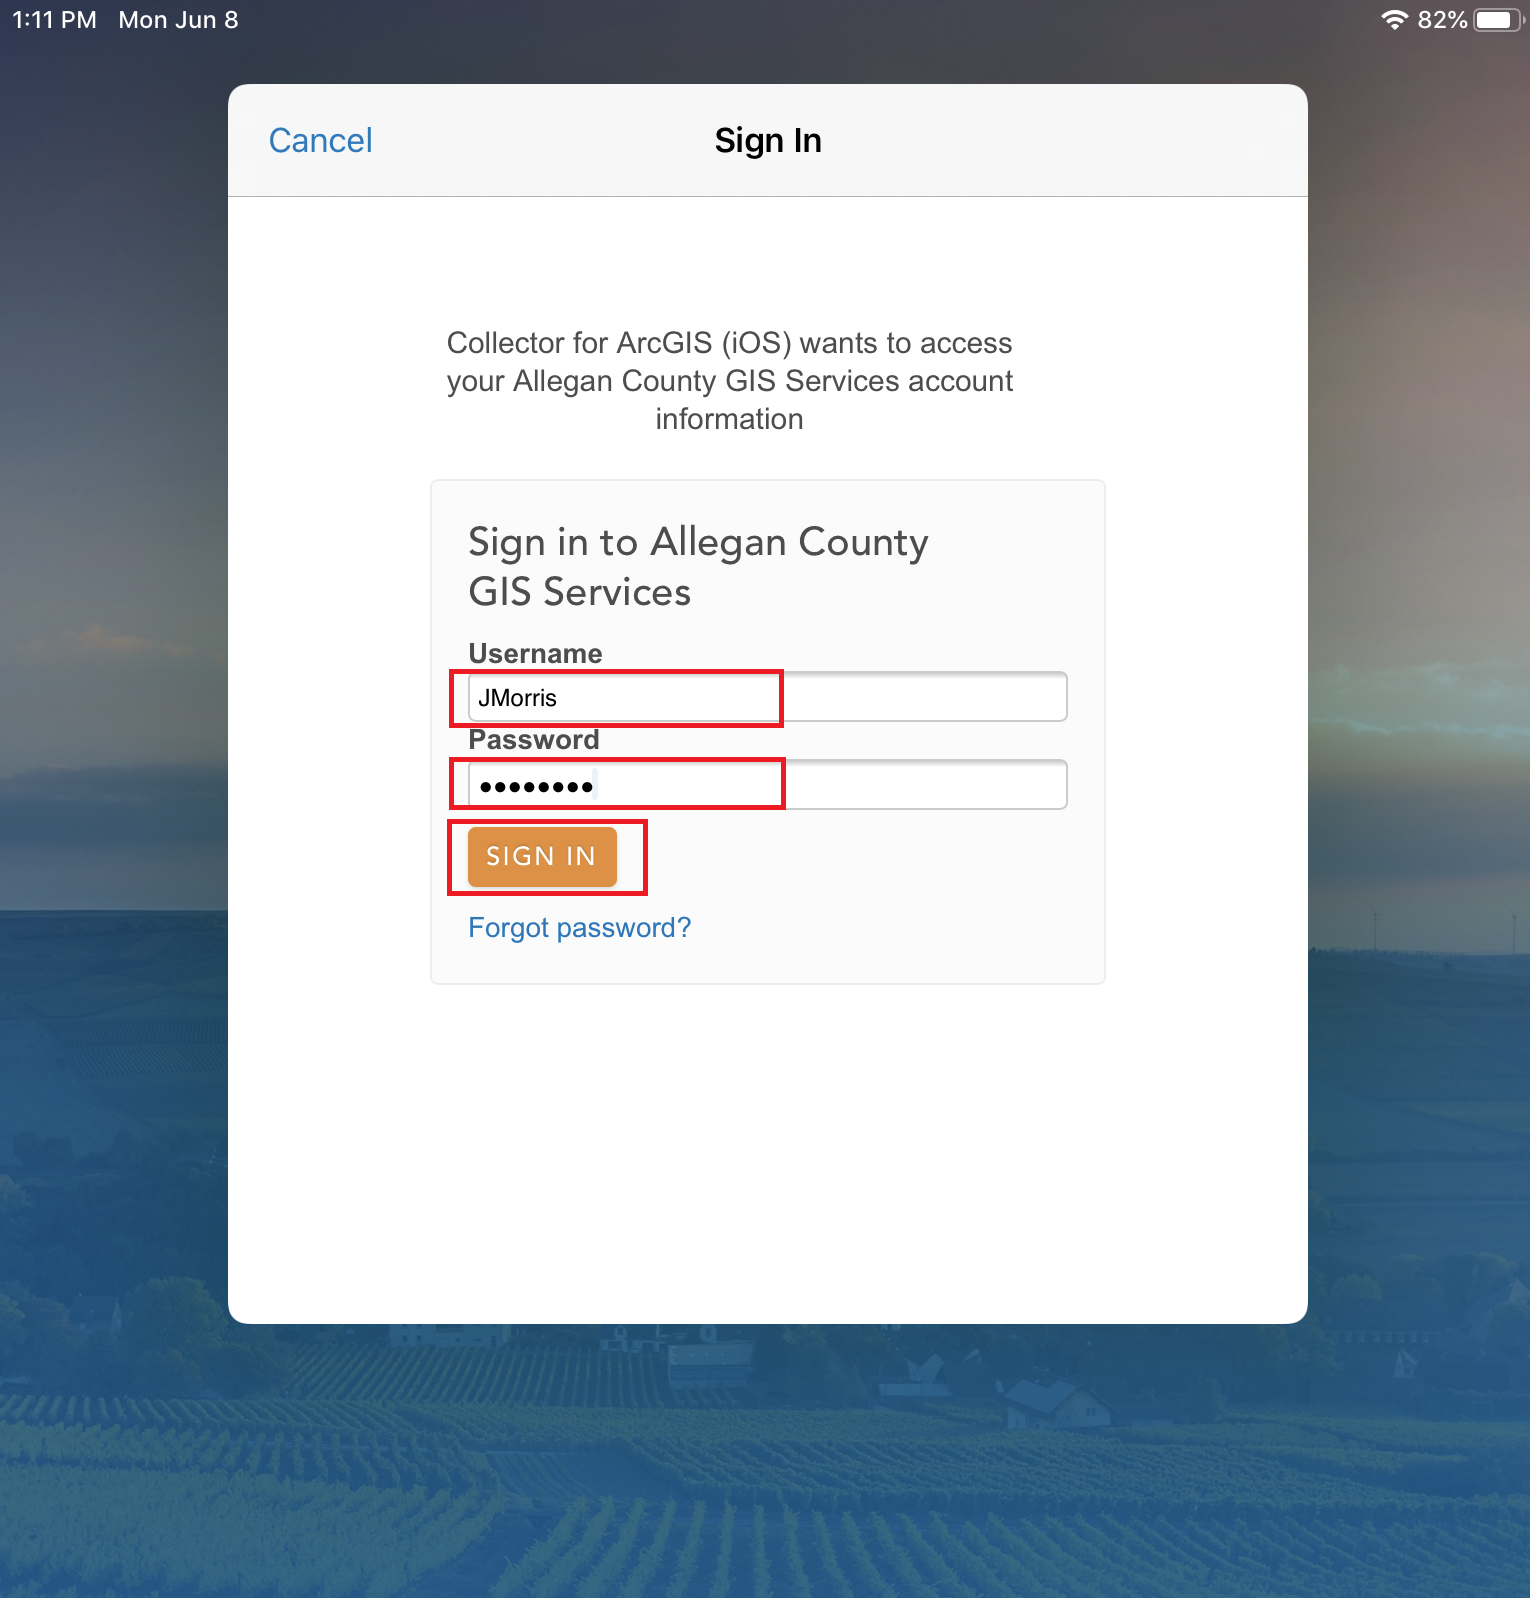
\includegraphics[width=.3\textwidth]{EnterCredentials.png}
\caption{Enter Credentials}
\end{wrapfigure}
for Organization Website, Type:
\vspace{.5in}

\begin{verbatim}
https://gis.allegancounty.org/
portal_webadaptor

\end{verbatim}

then:\\

Press Continue

\vspace{3in}
Enter Credentials\\

then:\\

Press SIGN IN
\clearpage
\subparagraph{Download the Forfeiture Field Map}

\subparagraph*{\\}
\begin{wrapfigure}{r}{0.5\textwidth}
\centering
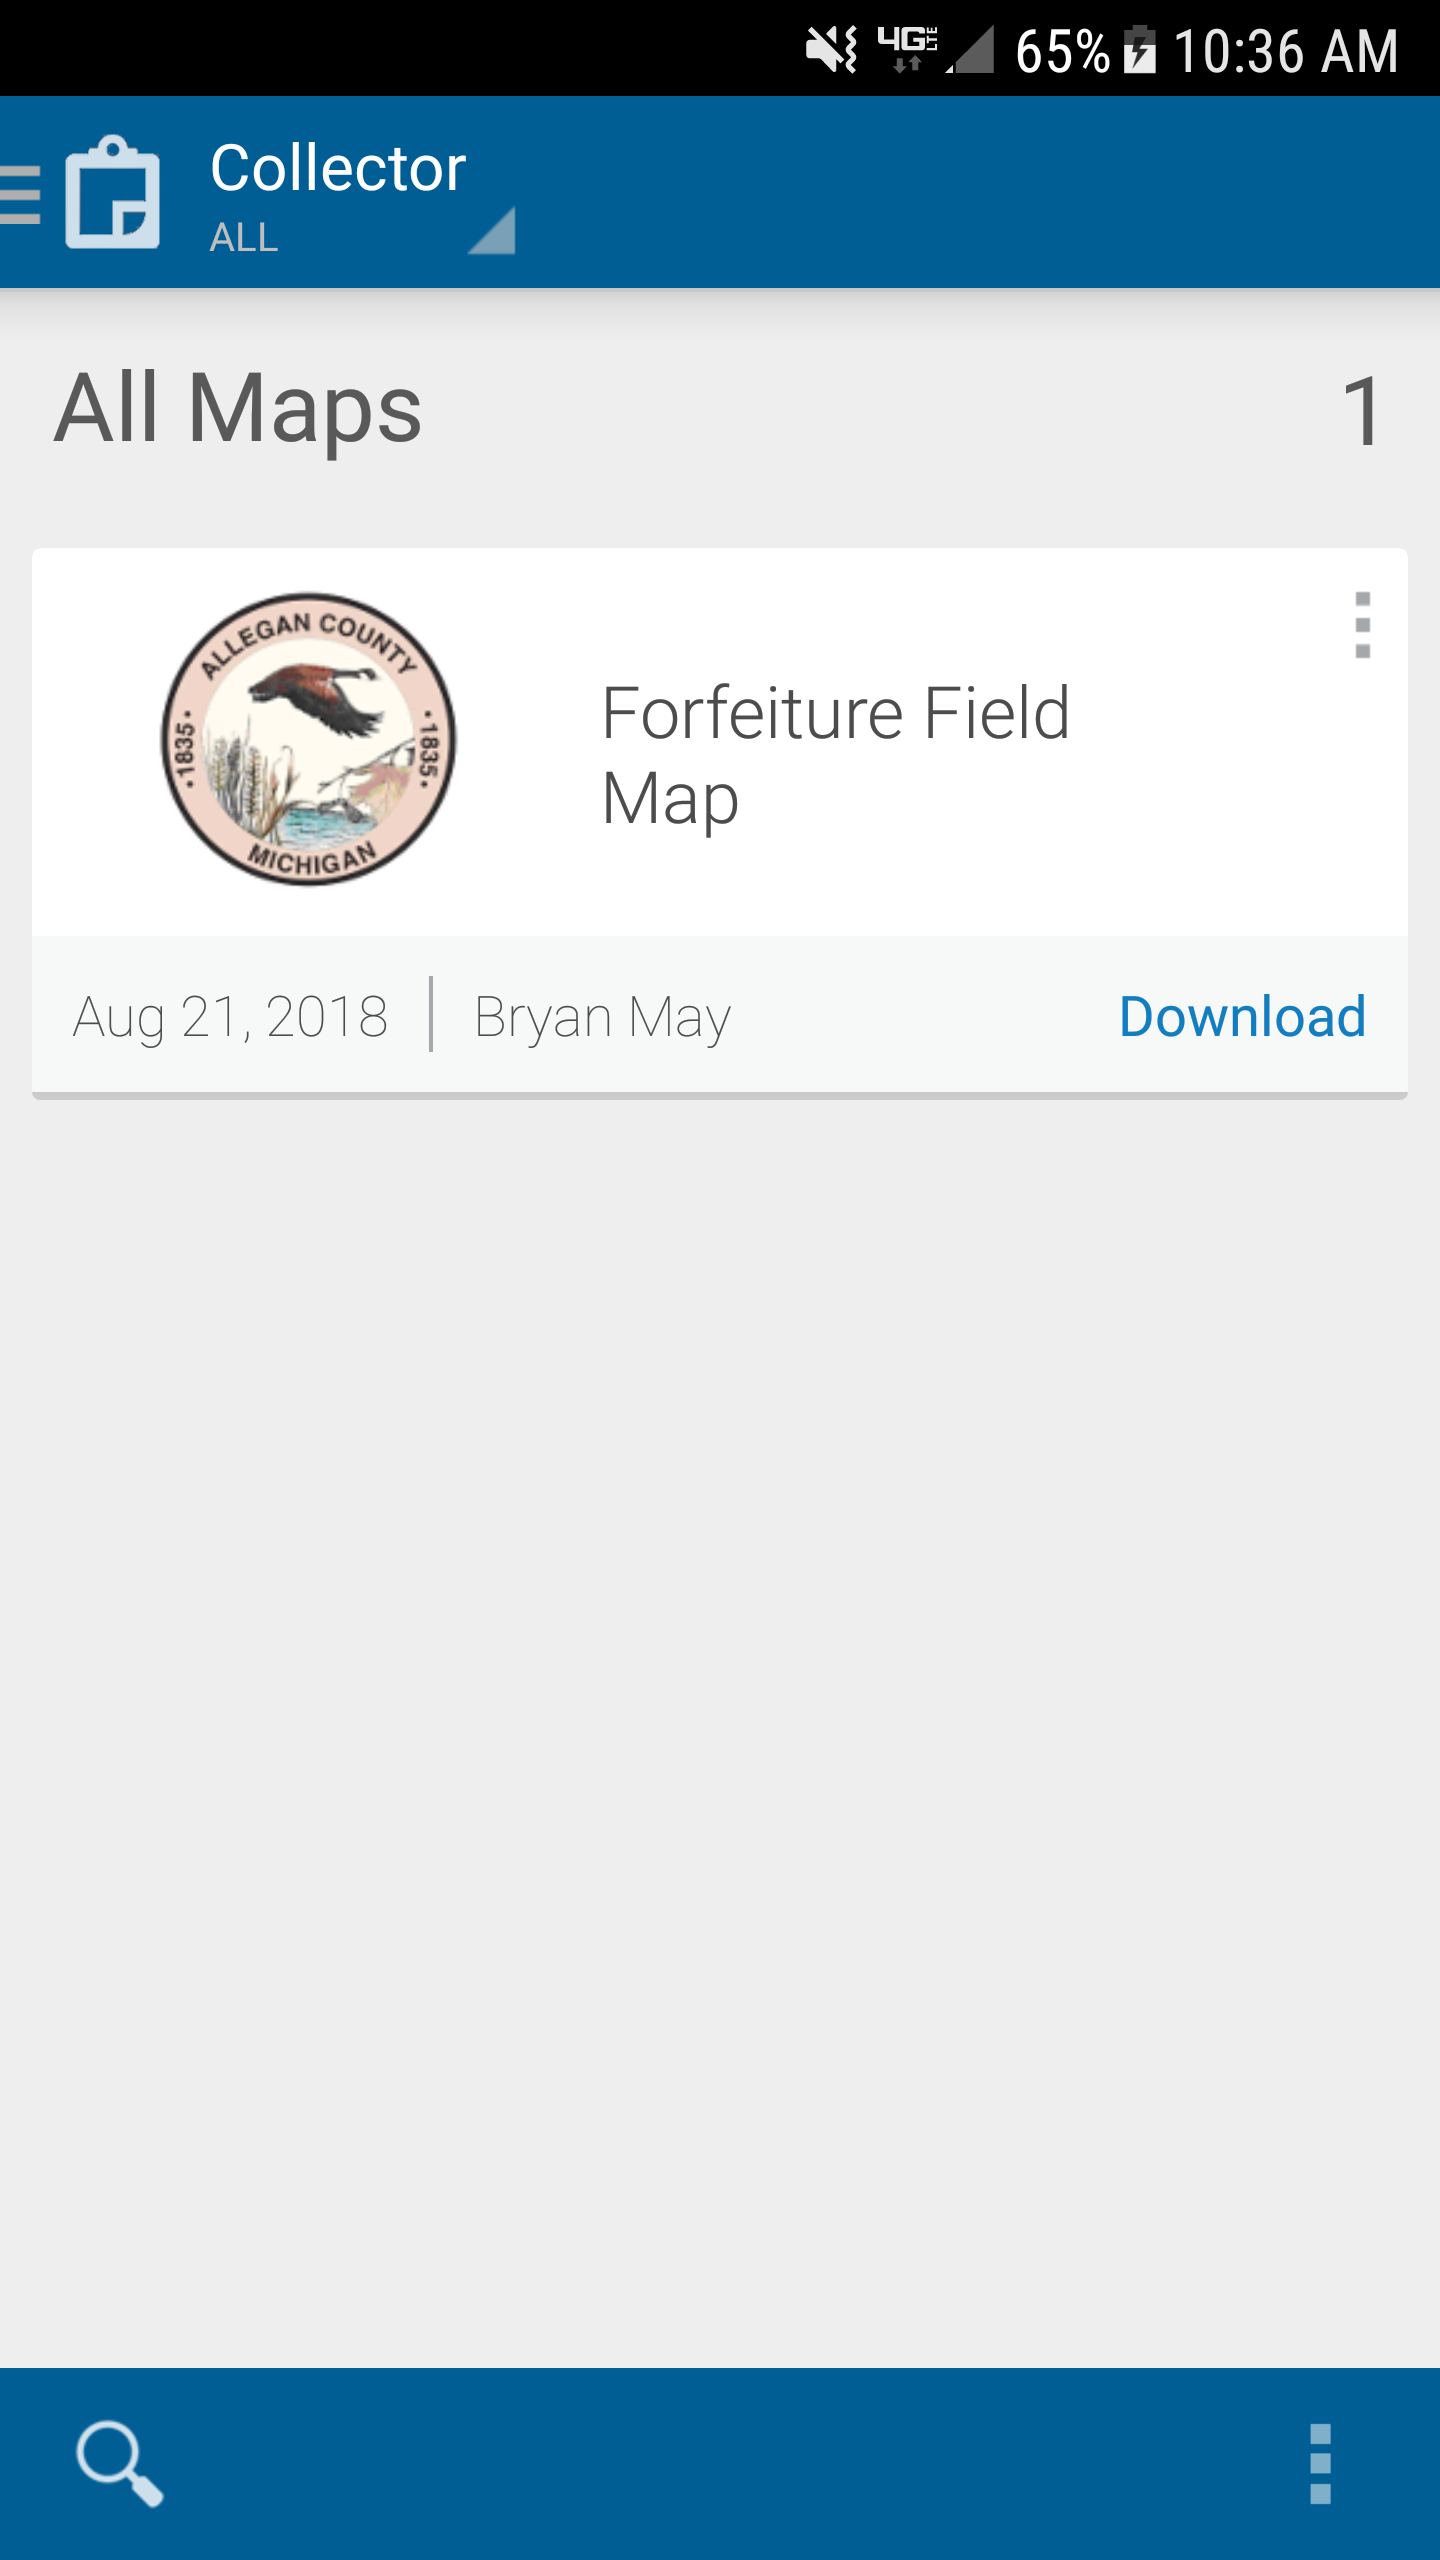
\includegraphics[width=.3\textwidth]{CollectorMapsMenu.png}
\caption{Collector Maps Menu}
\vspace{.25in}
\HRule \\[.4cm] % Horizontal Line added
\vspace{.25in}
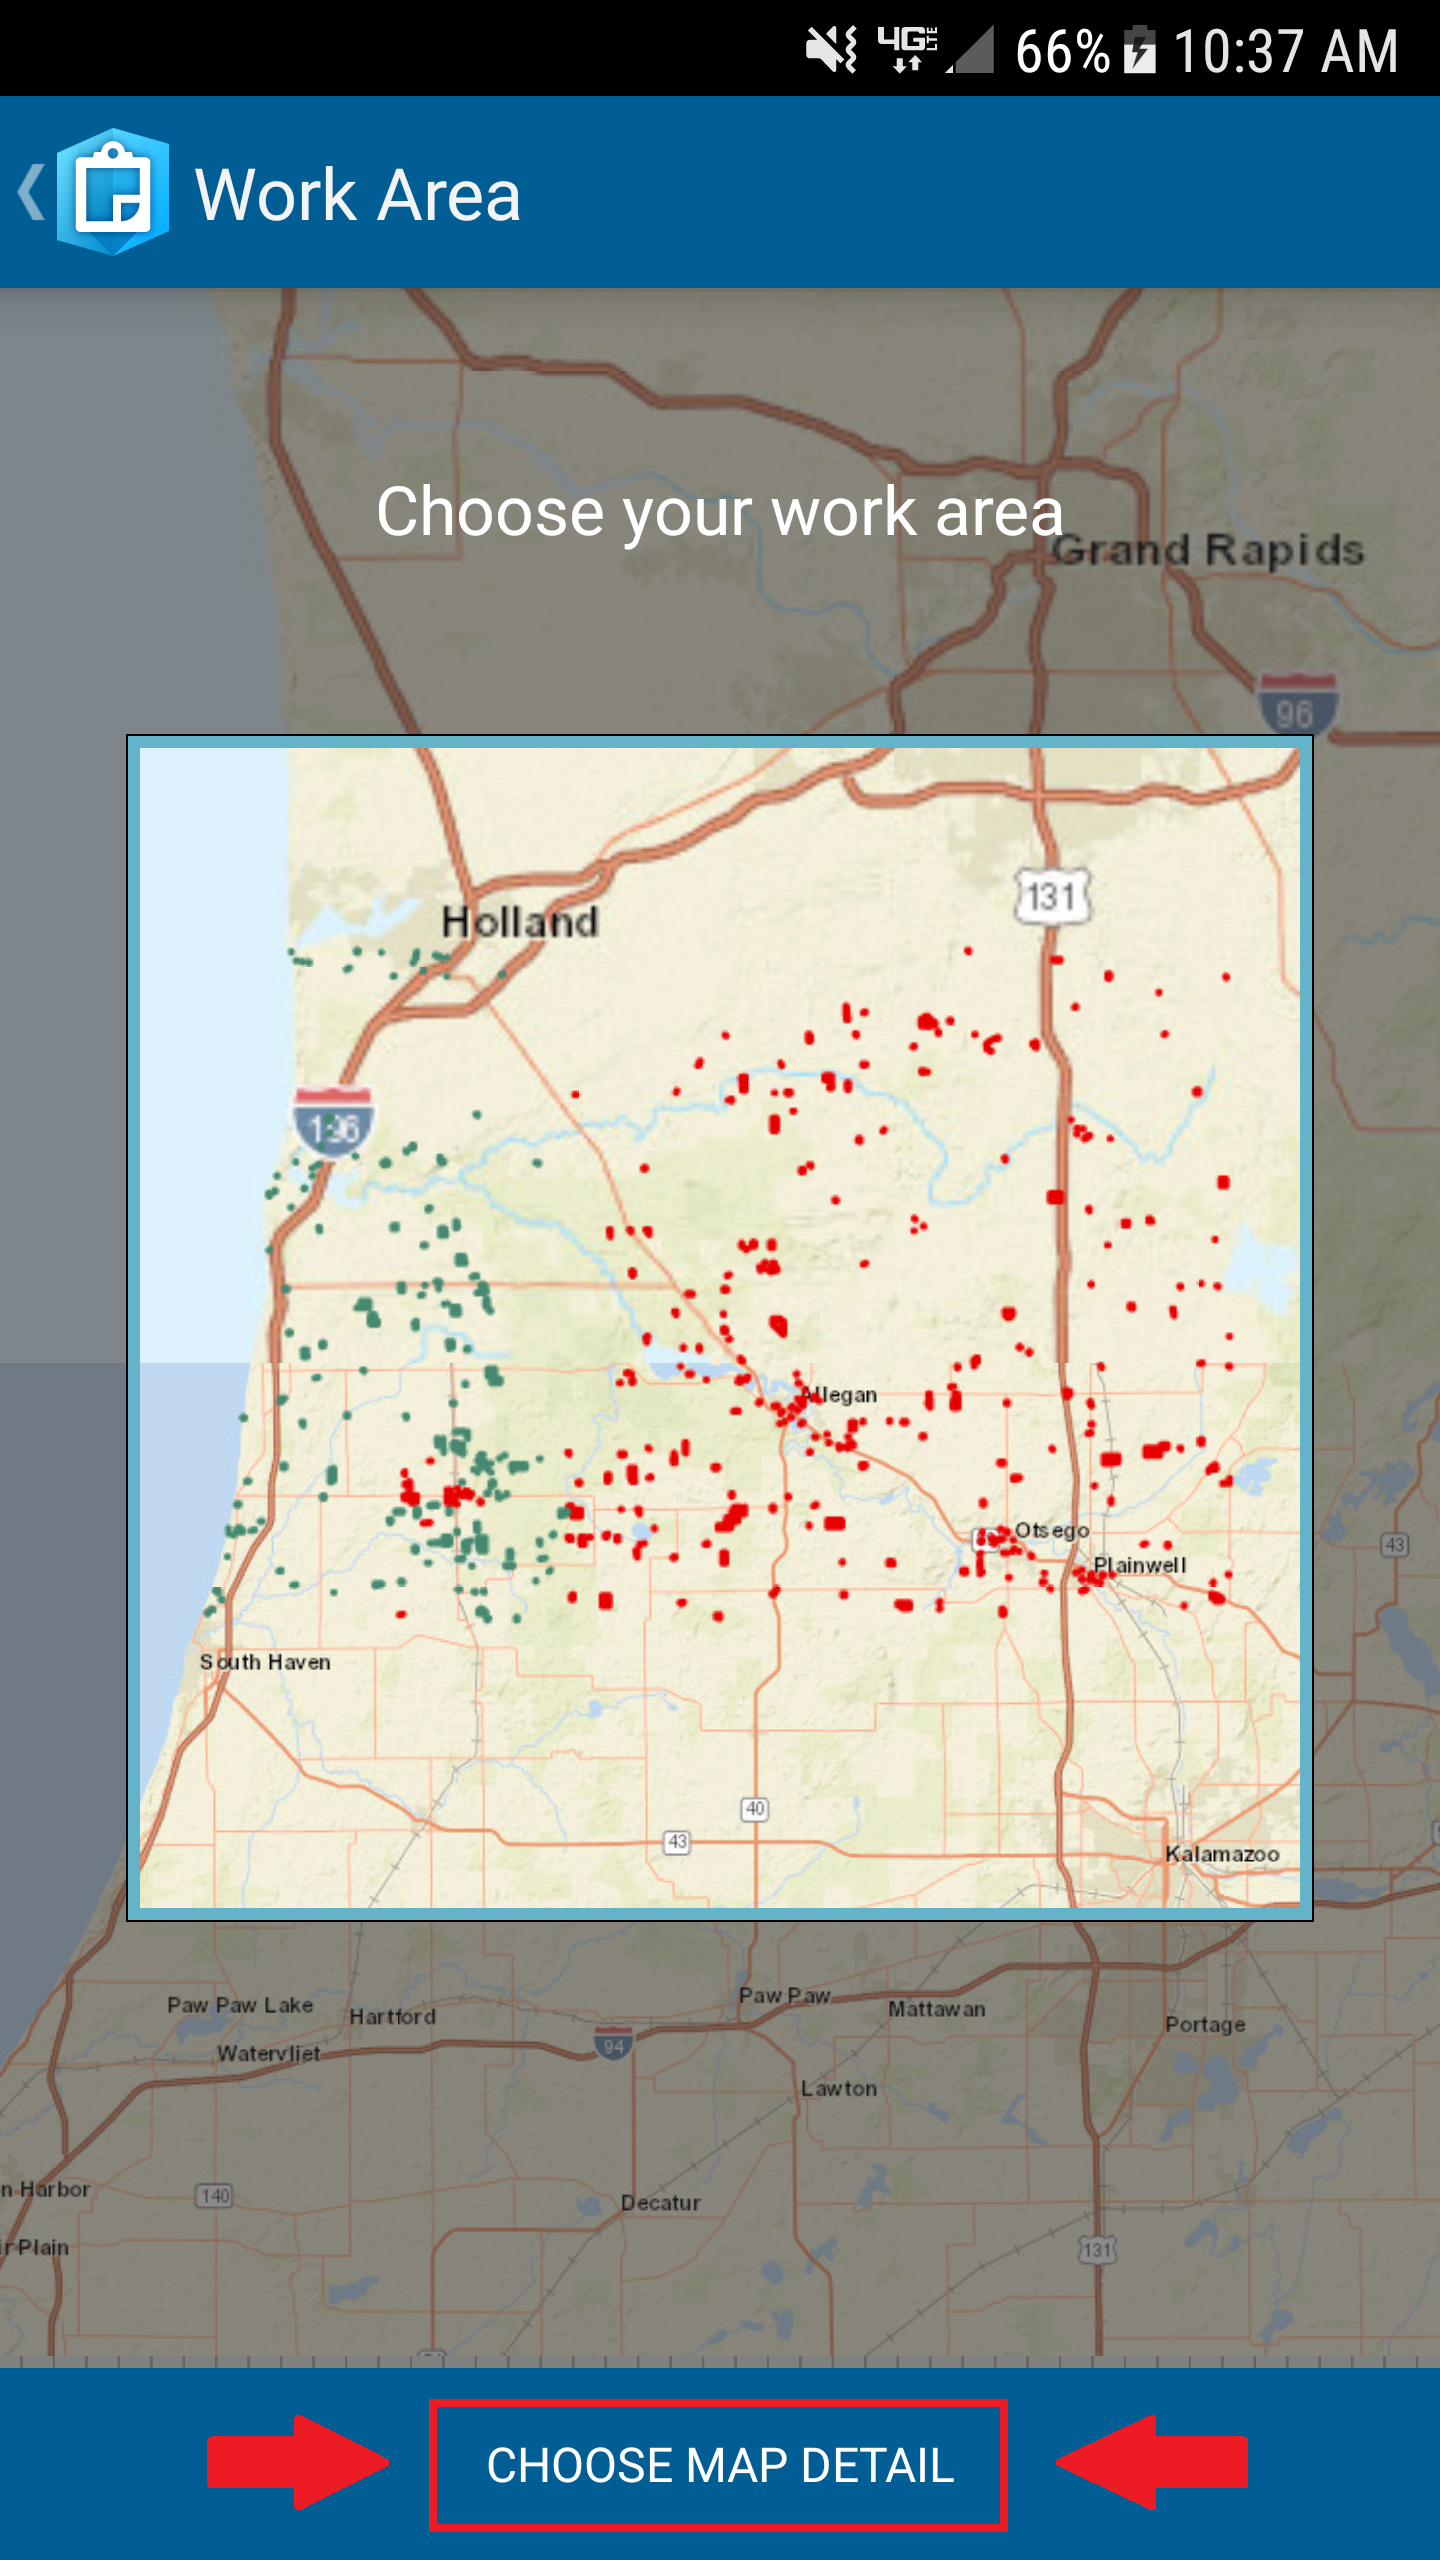
\includegraphics[width=.3\textwidth]{ChooseWorkAreaLarge.png}
\caption{Choose Work Area (large)}
\end{wrapfigure}
The Download option indicates it is not on the device but is available for offline use.
\vspace{.5in}

\noindent Press Download\\
\vspace{3in}

\noindent Specify work area to download\\
\vspace{1in}

\noindent \footnotesize Note that a larger area takes longer to download but the basemap only needs to be downloaded once.
\clearpage
\subparagraph{Choose Map Detail}

\subparagraph*{\\}
\begin{wrapfigure}{r}{0.5\textwidth}
\centering
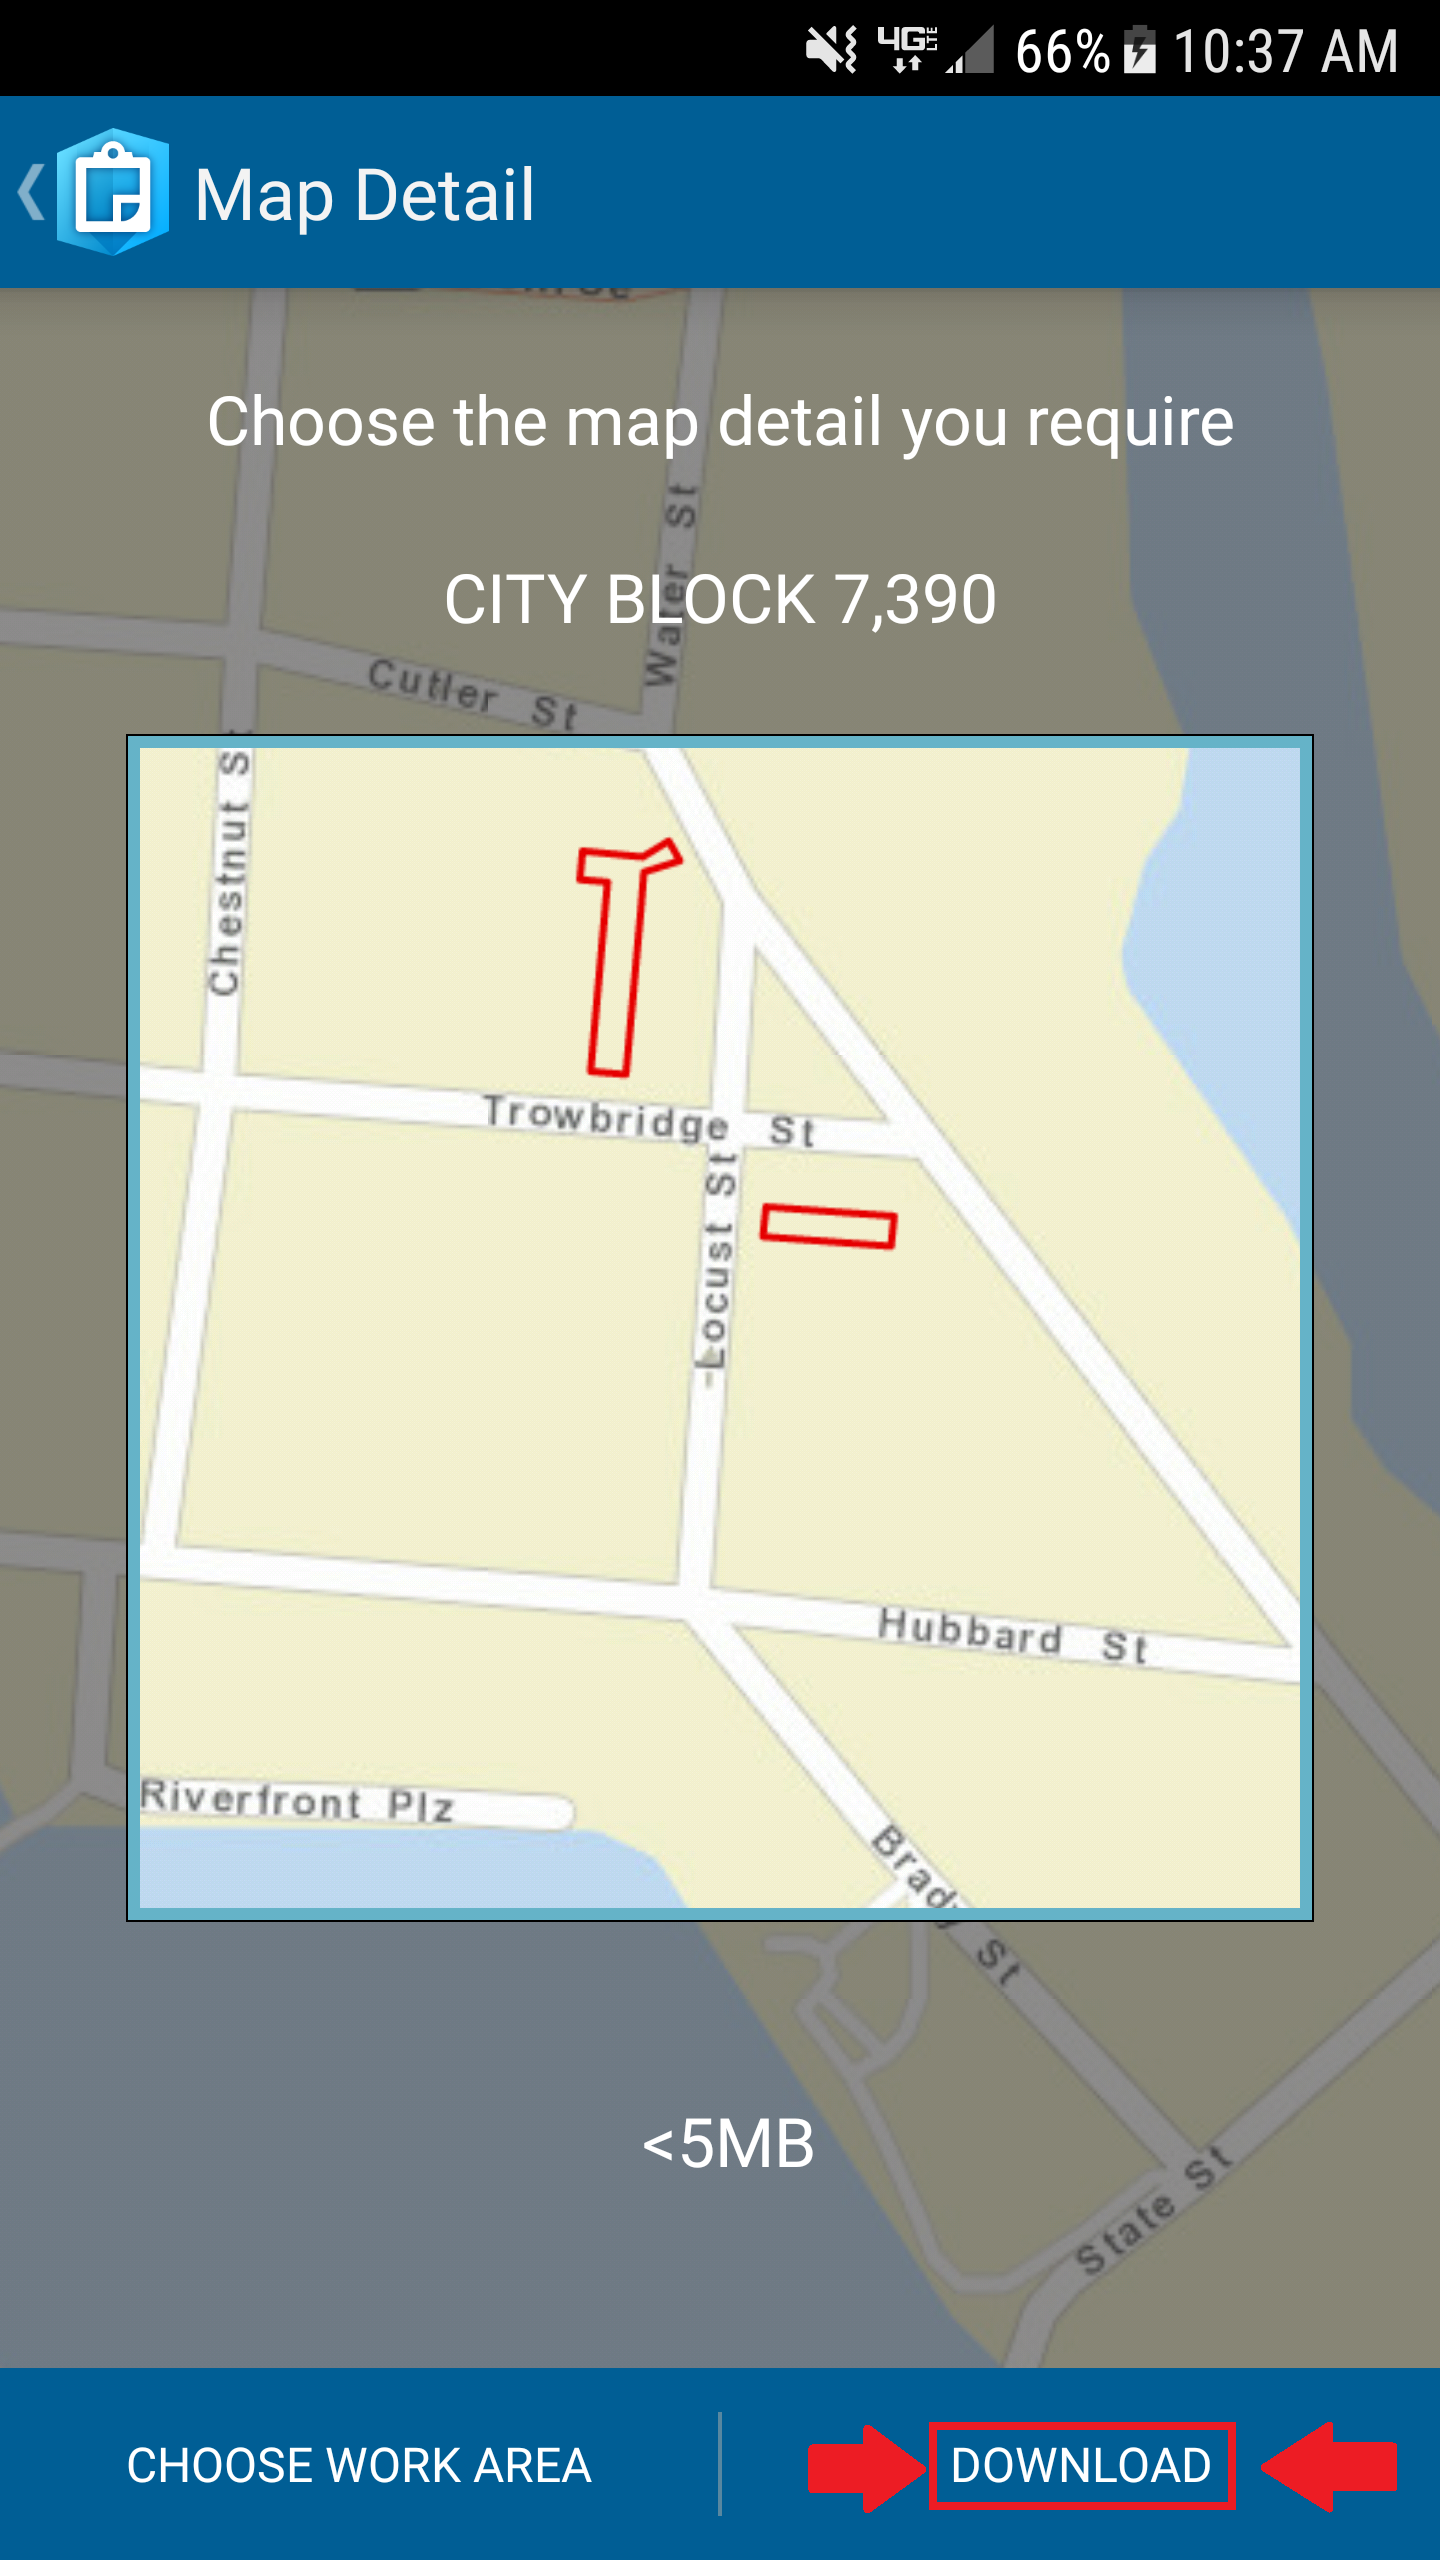
\includegraphics[width=.3\textwidth]{ChooseMapDetail.png}
\caption{Choose Map Detail}
\vspace{.25in}
\HRule \\[.4cm] % Horizontal Line added
\vspace{.25in}
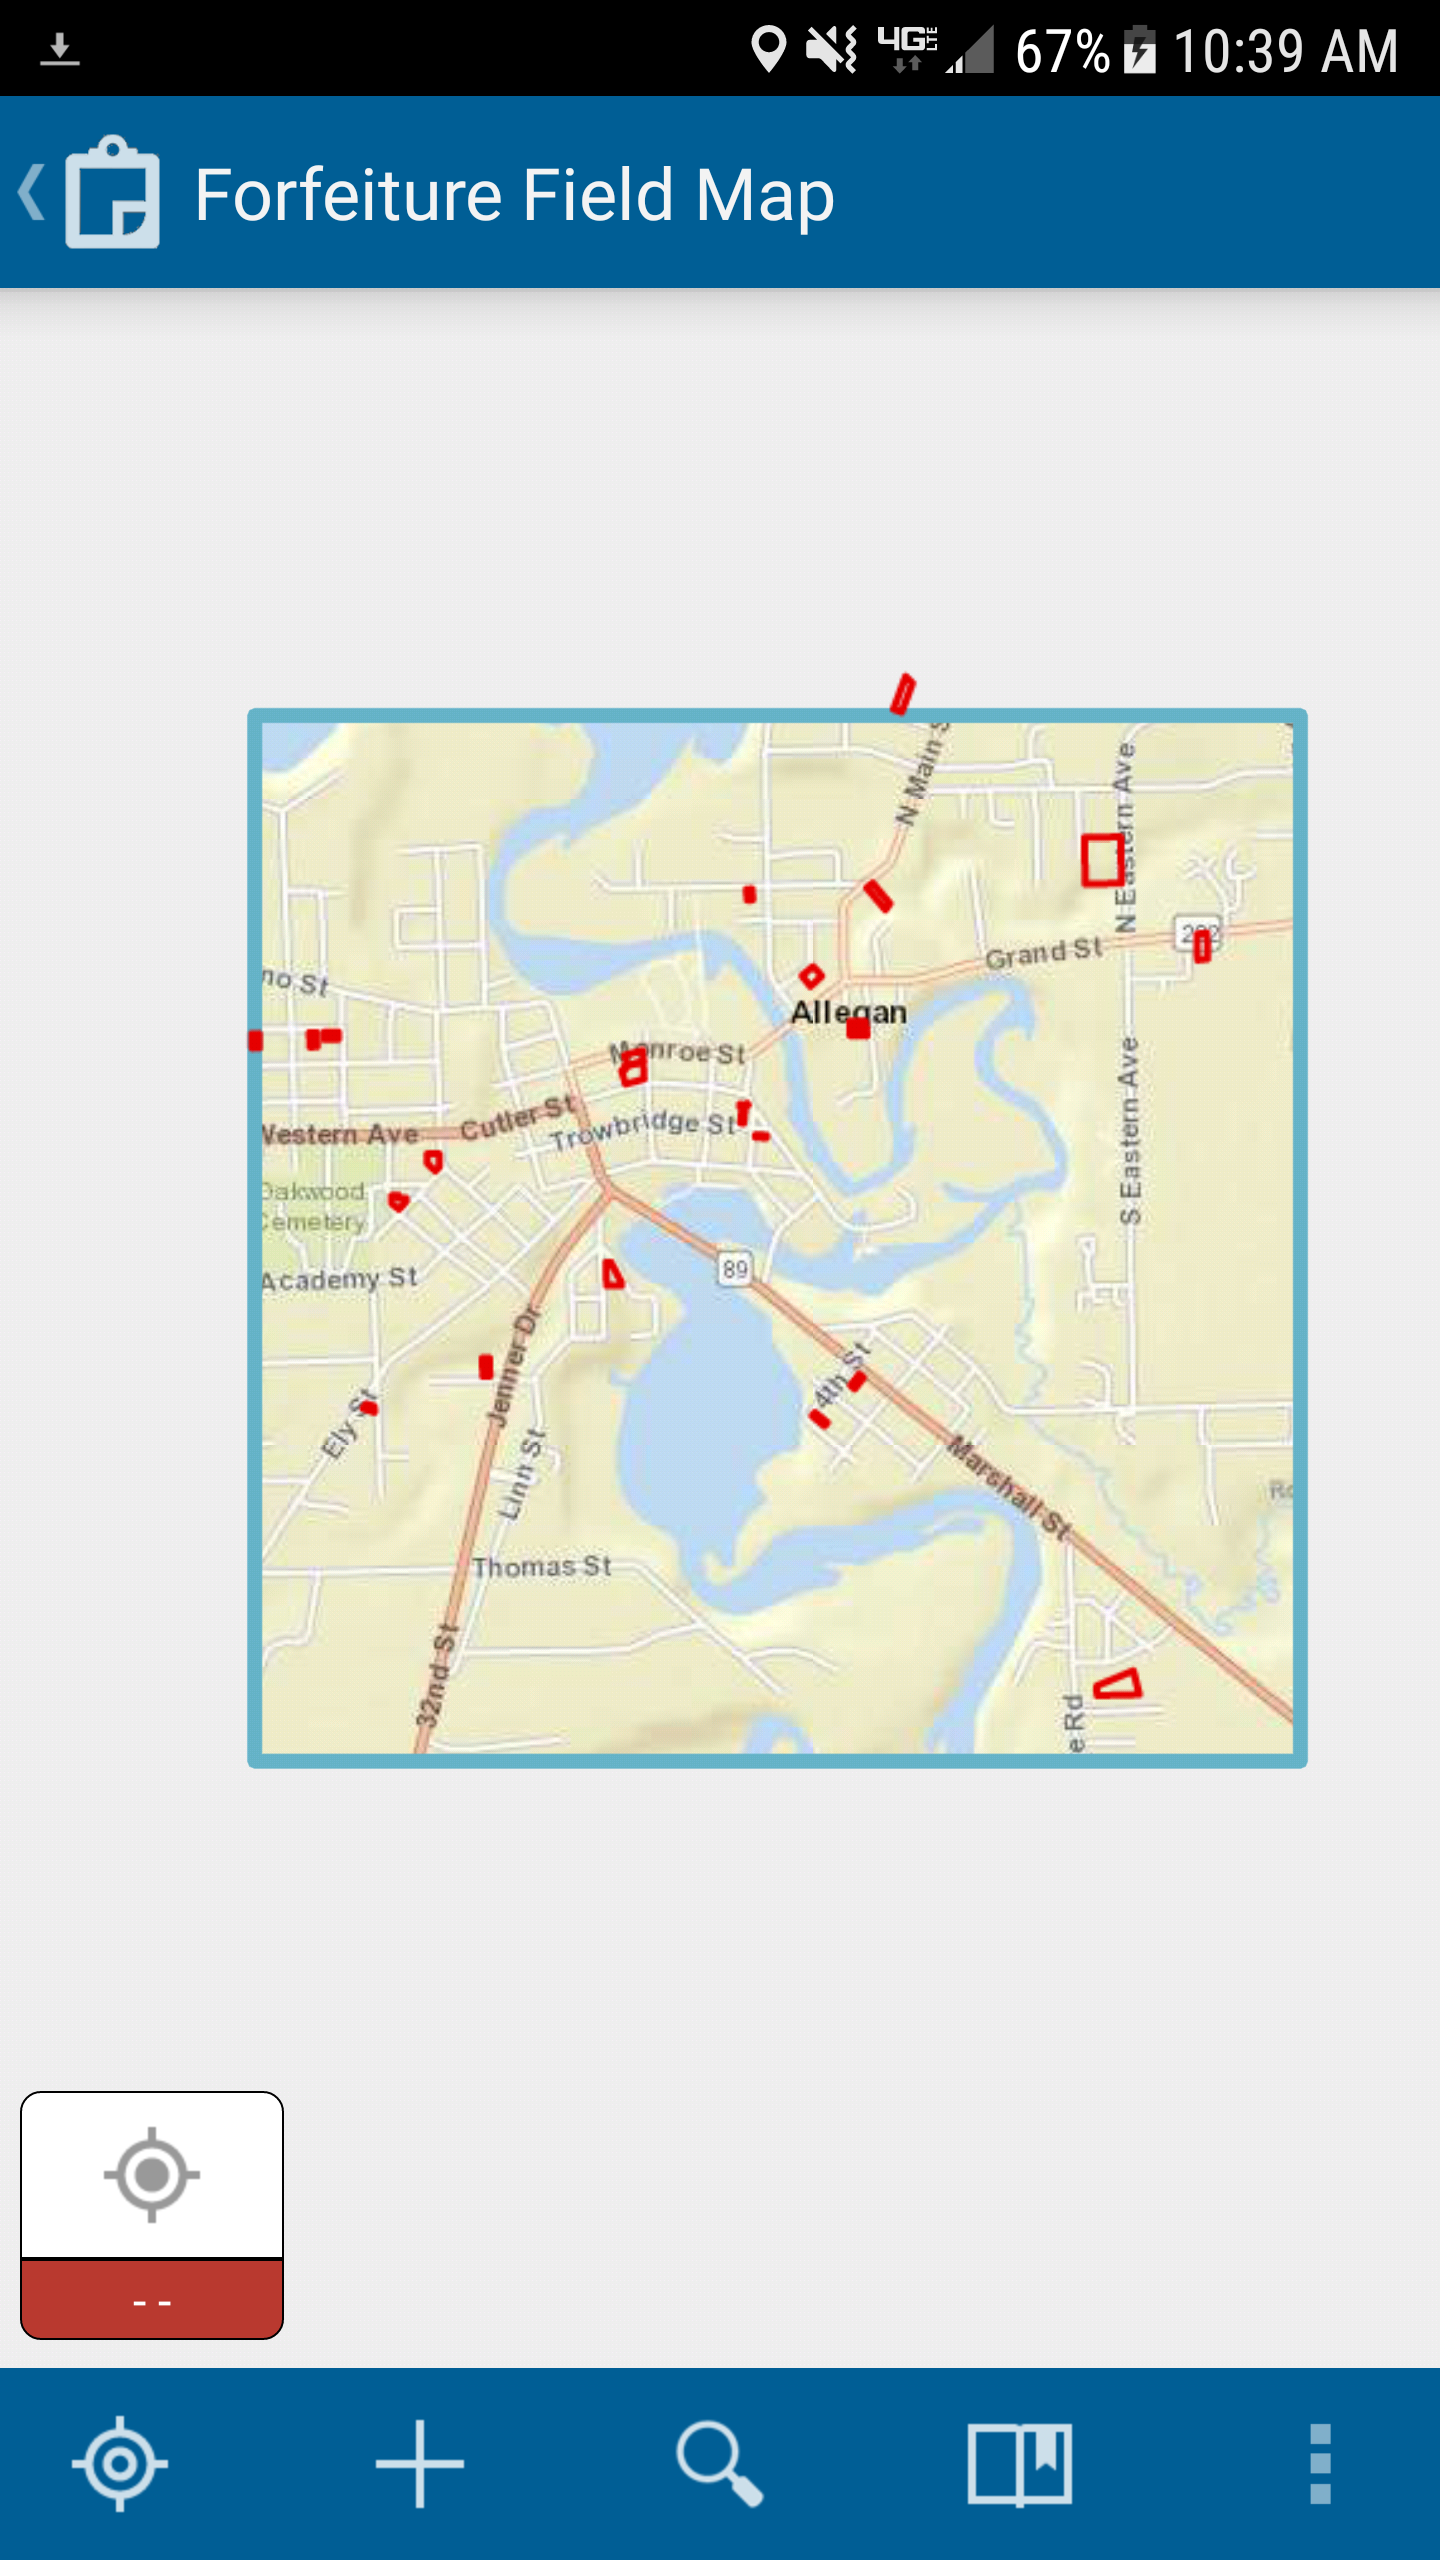
\includegraphics[width=.3\textwidth]{MaponDevice.png}
\caption{Map on Device}
\end{wrapfigure}
Zoom into the level of detail desired.
\vspace{.5in}

\noindent Press Download \\
\vspace{3in}

\noindent Here is how the map should look on the device:\\
\vspace{1in}

\noindent This area is ready for field data collection.
\clearpage


\paragraph{Daily Preprocessing Routine}

\subparagraph{Execute Preprocessing Script}A tool in ArcGIS that:

\begin{itemize}

\item Exports current forfeiture list from BSA
\item Updates webmap layers with results from BSA export

%Insert screenshot of Preprocesing script in Arc here

\end{itemize}

\clearpage
\subparagraph{Synchronize the Forfeiture Field Map\\}
\subparagraph*{\\}
\begin{wrapfigure}{r}{0.5\textwidth}
\centering
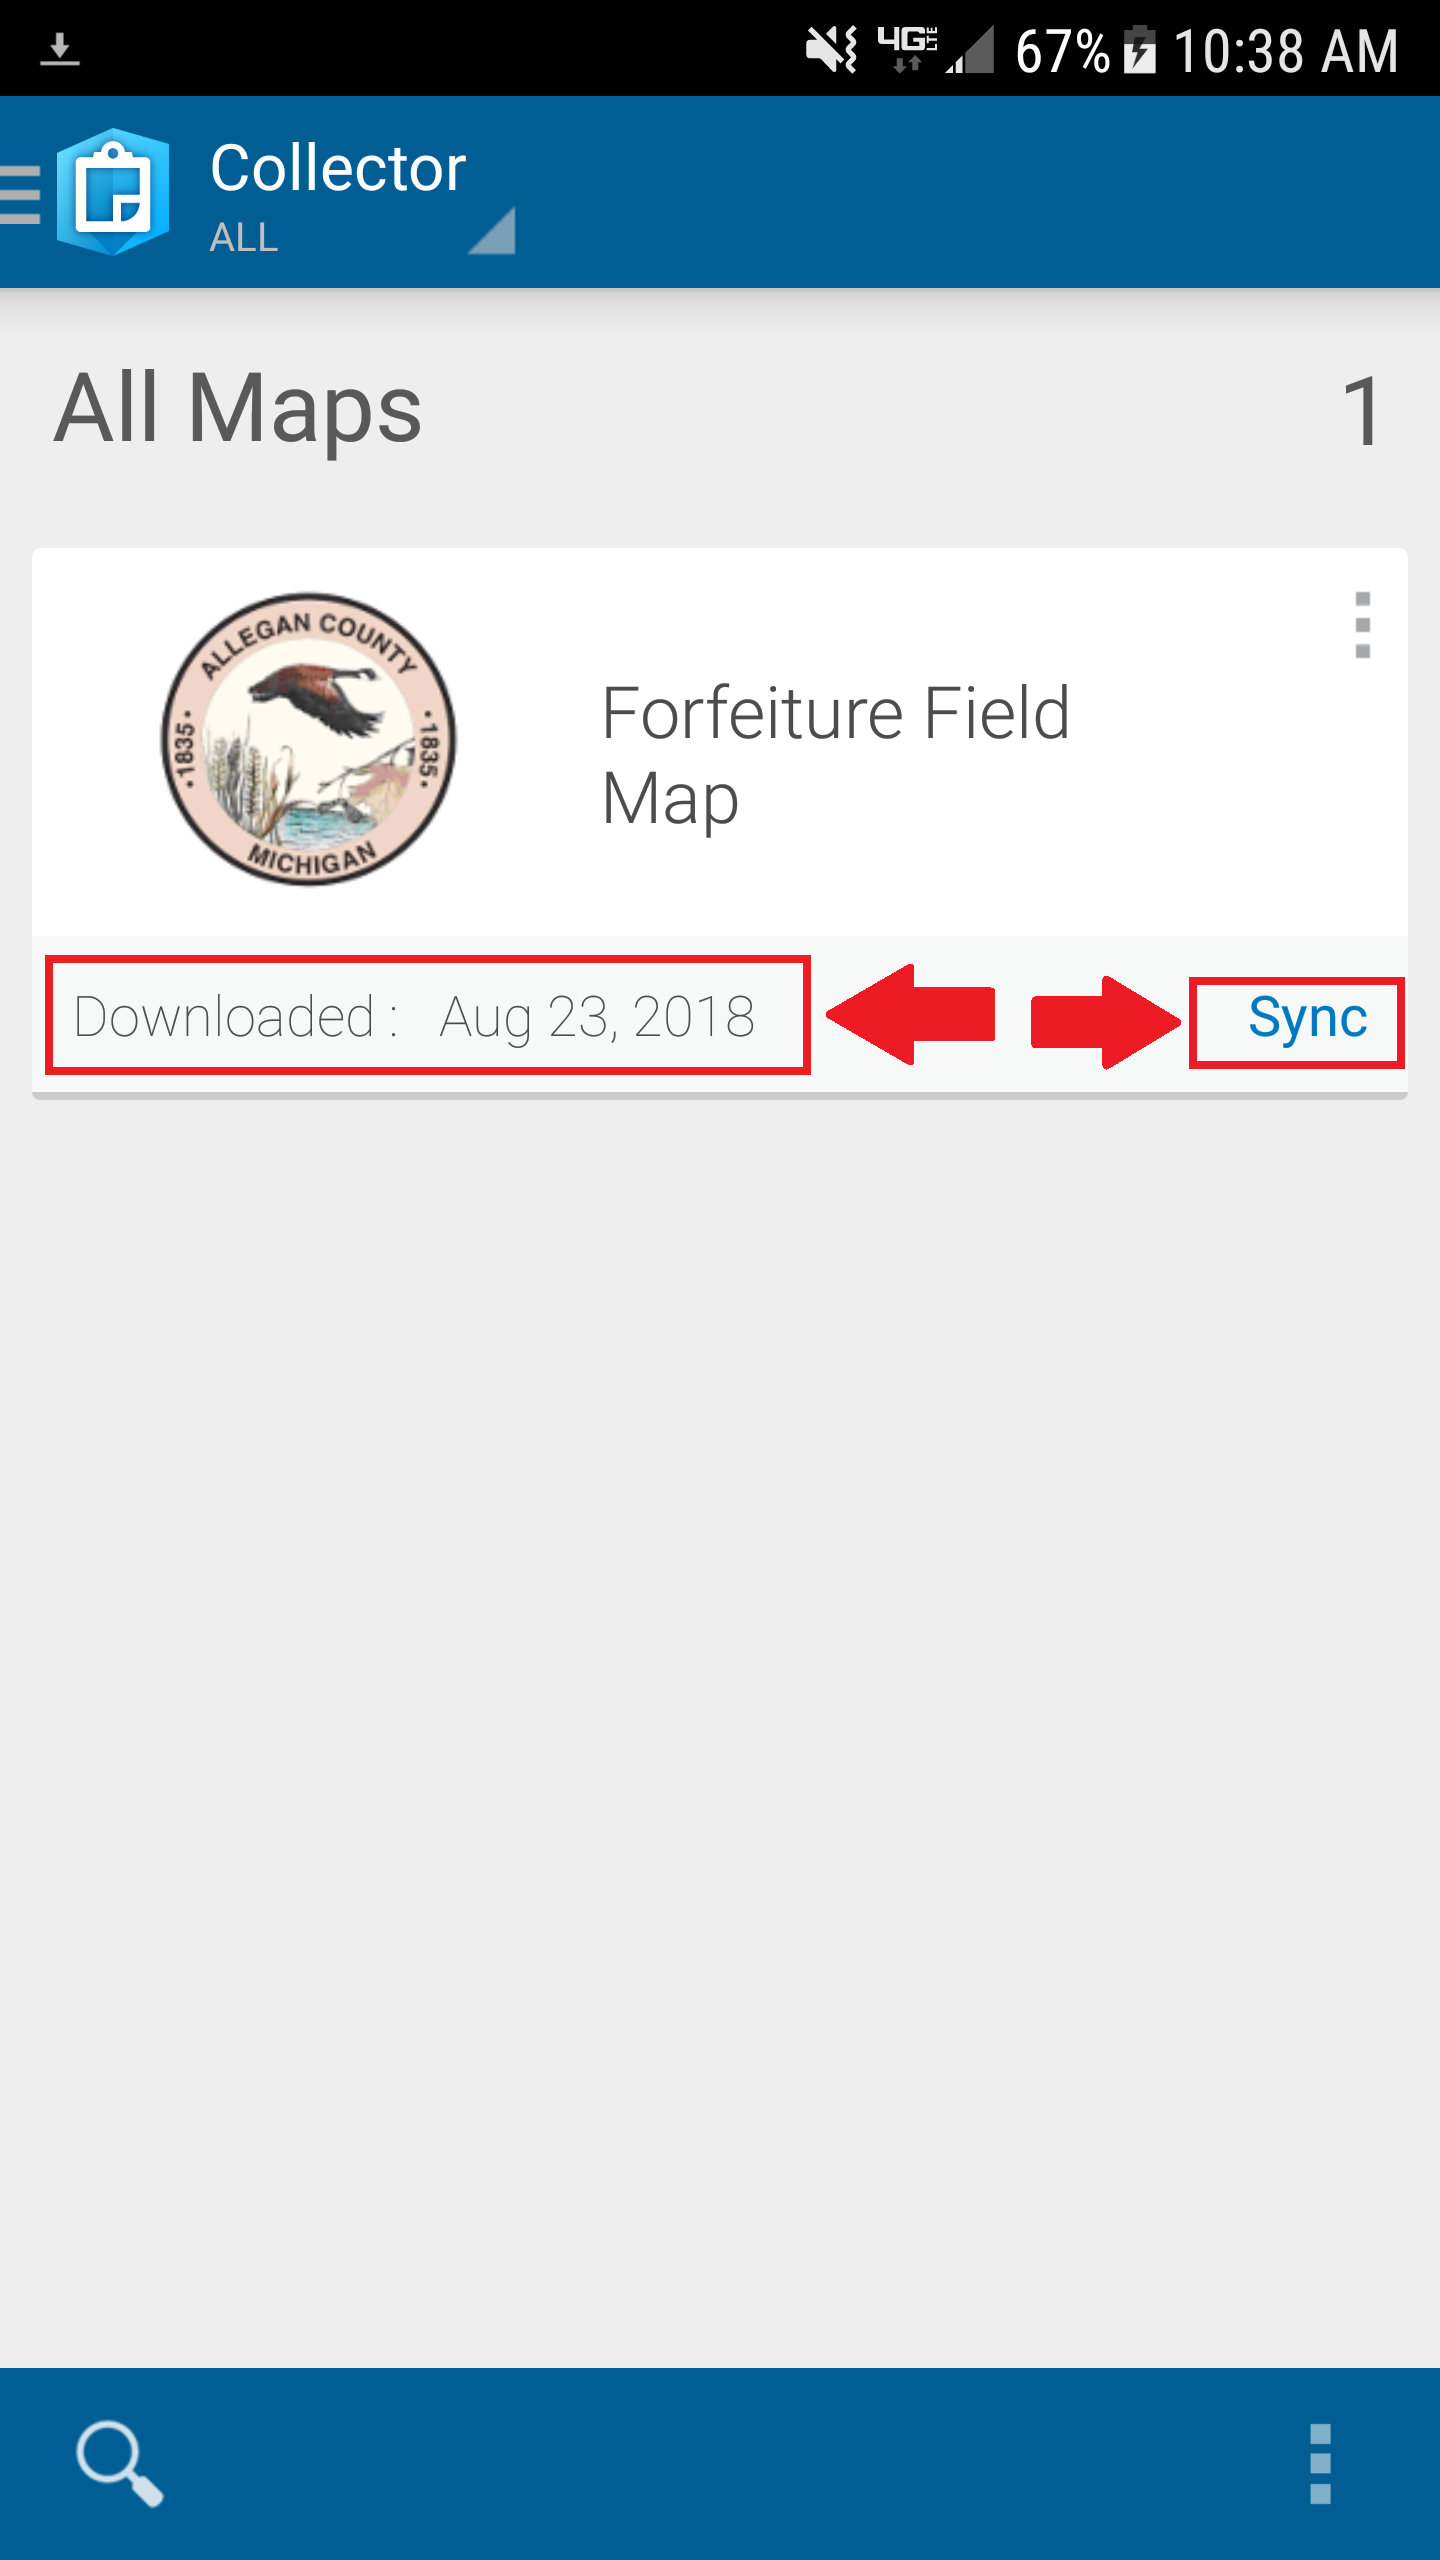
\includegraphics[width=.3\textwidth]{MapDownloaded.png}
\caption{Map Downloaded}
\vspace{.5in}
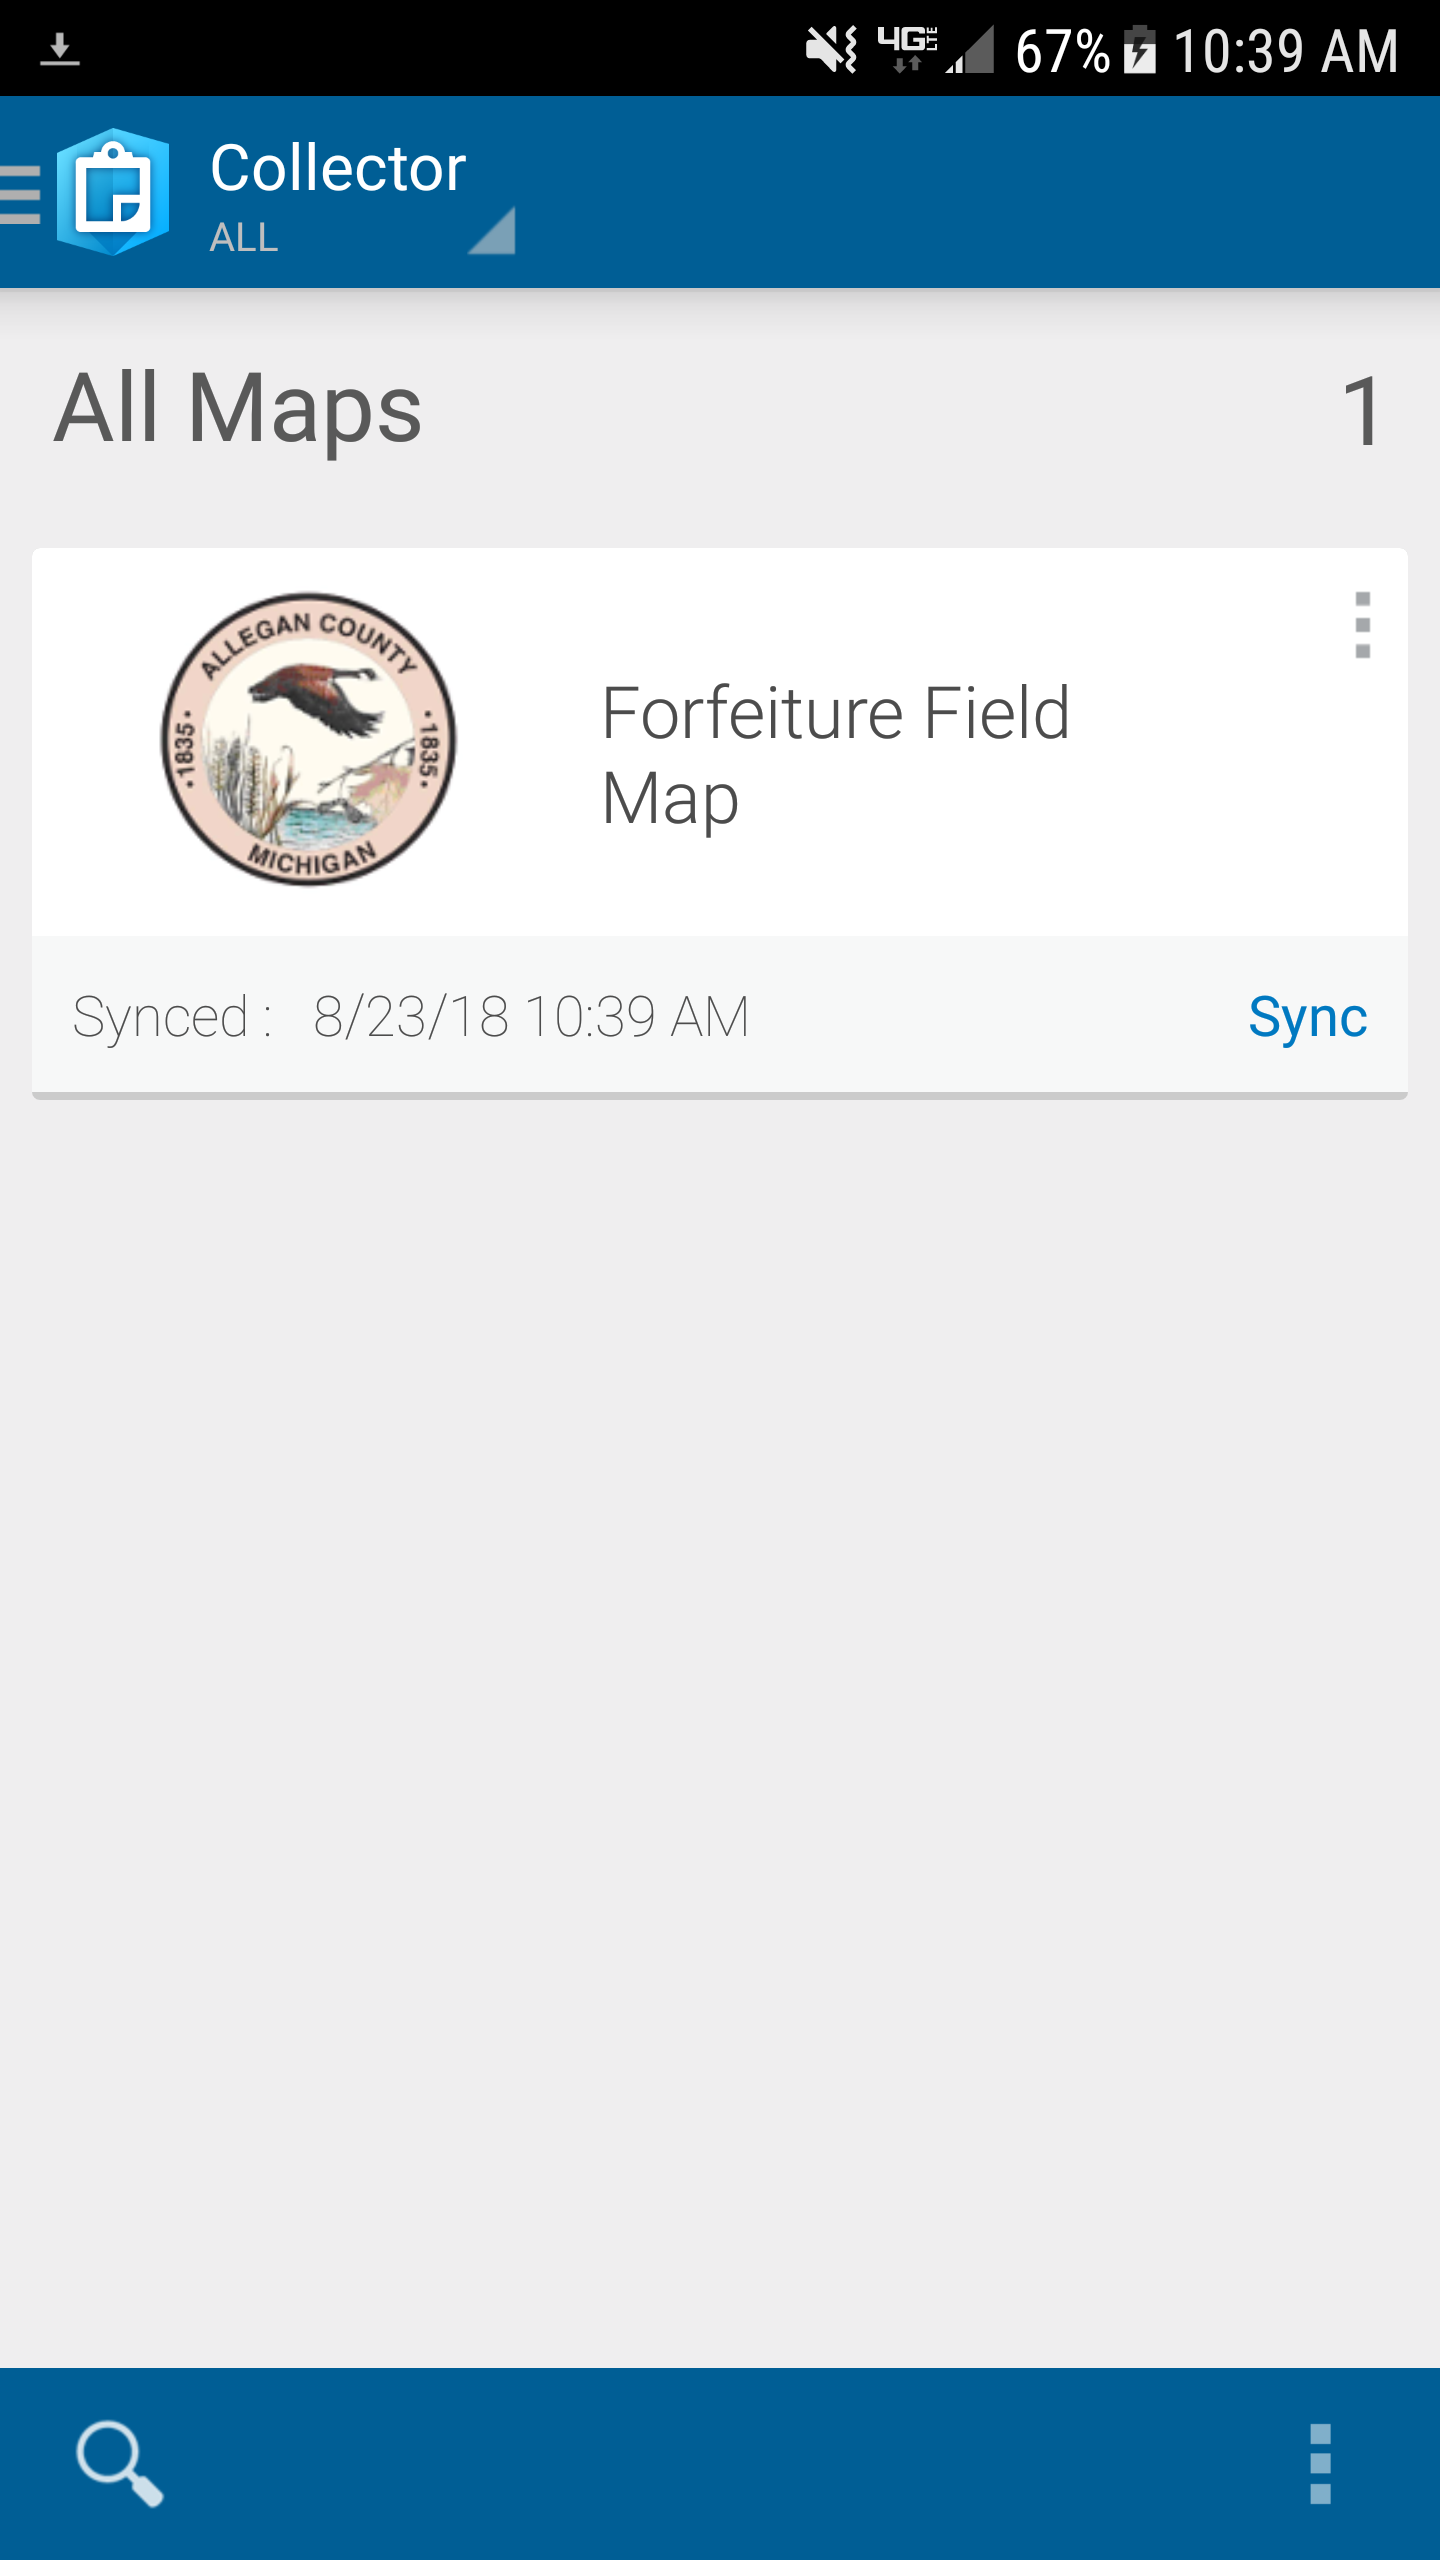
\includegraphics[width=.3\textwidth]{MapSyncronized.png}
\caption{Map Synchronized}
\end{wrapfigure}
Note the date and time:
\vspace{1.5in}

\noindent Press Sync
\vspace{1.5in}

Note the date and time\\

Map is now synchronized
\clearpage
\paragraph{Forfeiture Data Collection}
\subparagraph{Forfeiture Parcels Data Details}
Attributes are of four entry types:\begin{itemize}
\item prefilled
\item autofill
\item dropdown
\item text box \end{itemize}
In the Forfeiture Field Map, for each site visited, select the desired parcel, push the edit button and collect attributes.  If the boxes are autofill, select from dropdown or typed.\bigskip 
\begin{table}
\centering
\begin{tabular}{|l|c|r|}
\hline
\multicolumn{3}{|c|}{Attribute List} \\
\hline
Field Name&Entry Type&Note\\ \hline
Property Number&Prefilled&NA\\
Inspection Date&{\scriptsize Autofill or Dropdown}&NA\\
Inspector&Dropdown&NA\\
Class&Prefilled&NA\\
Acres&Prefilled&NA\\
Address&Prefilled&NA\\
Status&Dropdown&NA\\
Status Notes&Open entry&254 Char limit\\
Road Frontage&Dropdown&Yes or No\\
Access via&Open entry&30 Char Limit\\
Agent&Open entry&30 Char Limit\\
Agent Contact&Open entry&30 Char Limit\\
Property in use&Dropdown&Yes or\\
Use Notes&Open entry&254 Char limit\\
Property Maintained&Dropdown&Yes or No\\
Notes&Dropdown&254 Char limit\\
Prop Contam&Dropdown&Yes or No\\
Notes&Open entry&254 Char limit\\
Adj Prop Contam&Dropdown&NA\\
Notes&Open entry&254 Char limit\\
Property for sale&Dropdown&Yes or No\\
Posted&Prefilled&in Pre and Postproc\\
InList&Prefilled&in Preproc\\
PostedInList&Prefilled&in Preproc\\
Print Today&Dropdown&Yes or No\\ \hline
\end{tabular}
\caption{Dataset Details}
\end{table}

\clearpage
\subparagraph{Device 1 Field Operation}
\subparagraph*{}In the Forfeiture Field Map, for each site visited, select the desired parcel, push the edit button and then edit attributes.

\begin{wrapfigure}{r}{0.5\textwidth}
\centering
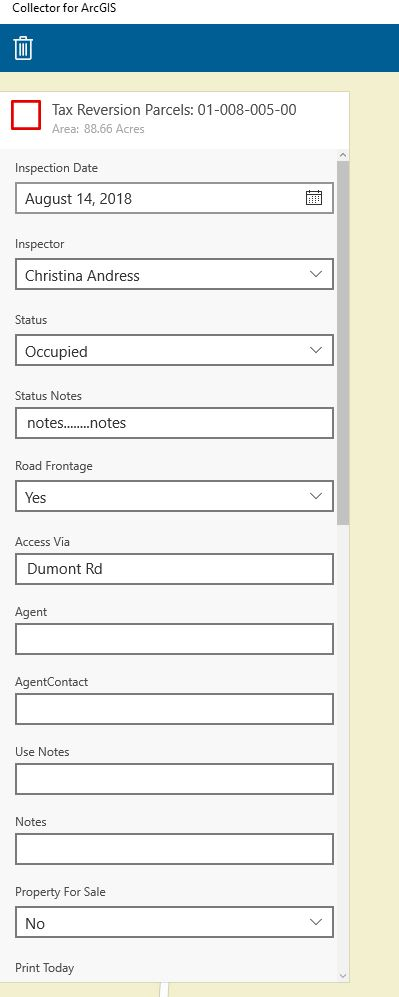
\includegraphics[width=.3\textwidth]{Device1DataEntry}
\caption {Device 1 Data Entry}
\end{wrapfigure}
\vspace{1in}

This figure shows the data collection interface.  Device one will be used to add data to all of the boxes.  Touch the boxes to enter text or select a dropdown.

\clearpage
\subparagraph{Device 2 Field Operation} 
\subparagraph*{}In the Forfeiture Field Map, for each site visited, select the desired parcel, push the edit button and then the add attachment button.  Select photo and take a photo.

\begin{wrapfigure}{l}{0.5\textwidth}
\centering
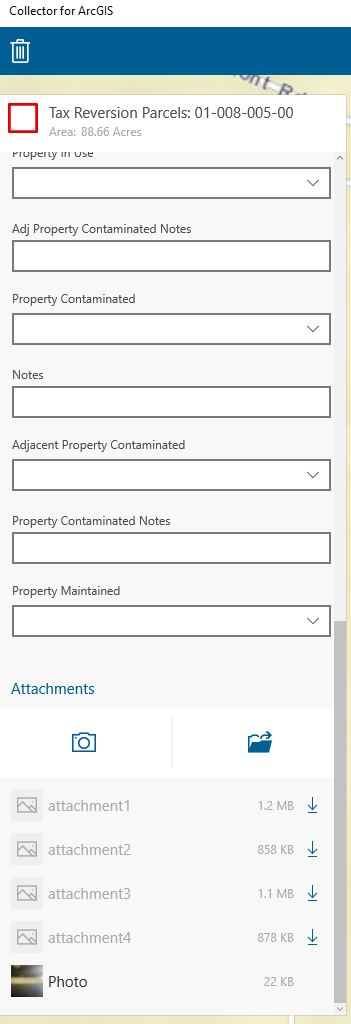
\includegraphics[width=.3\textwidth]{Device2DataEntry}
\caption {Device 2 Data Entry}
\end{wrapfigure}
\vspace{1in}

This figure shows the data collection interface.  Device two will be used to add photos to a parcel.

\clearpage
\paragraph{Daily Postprocessing Routine}Back at the office
\subparagraph{Synchronize Webmap}In Collector for ArcGIS, push the sync button on the Forfeiture Field Map
\subparagraph{Execute Postprocessing Script}A tool in ArcGIS that:

\begin{itemize}
\item Reconciles geodatabase versions
\item Generates forms for each site visited


%Insert screenshot of Postprocesing script in Arc here

\end{itemize}

%\begin{description}
%\item [Sync Edits] \blindtext
%\item [reconcile Versions] \blindtext
%\item[Print forms for site visits] \blindtext
%\item[Update BSA] \blindtext
%\end{description}

\clearpage
\subsubsection{Software}
\paragraph{ESRI Licensed Products}
\subparagraph{ArcDesktop}Users of this application need a license to ArcGIS Standard level.

\subparagraph{Enterprise ArcGIS Deployment}This app uses ArcGIS Server and ArcGIS Portal.

\subparagraph{Collector for ArcGIS}Developed and tested on Android(7.0).  Collector is available at the Google Play Store.

\end{document}